%%%%%%%%%%%%%%%%%%%%%%%%%%%%%%%%%%%%%%%%%
% Journal Article
% LaTeX Template
% Version 1.3 (9/9/13)
%
% This template has been downloaded from:
% http://www.LaTeXTemplates.com
%
% Original author:
% Frits Wenneker (http://www.howtotex.com)
%
% License:
% CC BY-NC-SA 3.0 (http://creativecommons.org/licenses/by-nc-sa/3.0/)
%
%%%%%%%%%%%%%%%%%%%%%%%%%%%%%%%%%%%%%%%%%

%----------------------------------------------------------------------------------------
%	PACKAGES AND OTHER DOCUMENT CONFIGURATIONS
%----------------------------------------------------------------------------------------

\documentclass[twoside]{article}
\usepackage{graphicx}
\graphicspath{ {./Col_esc_Figures/} }
\usepackage{lipsum} % Package to generate dummy text throughout this template
\usepackage{wrapfig}
\usepackage[sc]{mathpazo} % Use the Palatino font

\usepackage{amsmath}
\usepackage[T1]{fontenc} % Use 8-bit encoding that has 256 glyphs
\linespread{1.50} % Line spacing - Palatino needs more space between lines
\usepackage{microtype} % Slightly tweak font spacing for aesthetics
\usepackage{lineno}
\usepackage{putex}
\usepackage[hmarginratio=1:1,top=32mm,columnsep=20pt]{geometry} % Document margins
\usepackage{multicol} % Used for the two-column layout of the document
\usepackage[hang, small,labelfont=bf,up,textfont=it,up]{caption} % Custom captions under/above floats in tables or figures
\usepackage{booktabs} % Horizontal rules in tables
\usepackage{float} % Required for tables and figures in the multi-column environment - they need to be placed in specific locations with the [H] (e.g. \begin{table}[H])
\usepackage{hyperref} % For hyperlinks in the PDF
\usepackage{lettrine} % The lettrine is the first enlarged letter at the beginning of the text
\usepackage{paralist} % Used for the compactitem environment which makes bullet points with less space between them

%\usepackage{abstract} % Allows abstract customization
%\renewcommand{\abstractnamefont}{\normalfont\bfseries} % Set the "Abstract" text to bold
%\renewcommand{\abstracttextfont}{\normalfont\small\itshape} % Set the abstract itself to small italic text
\usepackage{newtxtext,newtxmath}
\usepackage{titlesec} % Allows customization of titles
\renewcommand\thesection{\Roman{section}} % Roman numerals for the sections
\renewcommand\thesubsection{\Roman{subsection}} % Roman numerals for subsections
\titleformat{\section}[block]{\large\scshape\centering}{\thesection.}{1em}{} % Change the look of the section titles
\titleformat{\subsection}[block]{\large}{\thesubsection.}{1em}{} % Change the look of the section titles

%\usepackage{fancyhdr} % Headers and footers
%\pagestyle{fancy} % All pages have headers and footers
%\fancyhead{} % Blank out the default header
%\fancyfoot{} % Blank out the default footer
%\fancyhead[C]{RCM $\bullet$ November 18$^{th}$ 2014 $\bullet$ Vol. XXI, No. 1} % Custom header text
%\fancyfoot[RO,LE]{\thepage} % Custom footer text

%----------------------------------------------------------------------------------------
%	TITLE SECTION
%----------------------------------------------------------------------------------------

\title{\vspace{-15mm}\fontsize{24pt}{10pt}\selectfont\textbf{Creating high-resolution maps of leaf water isotopes using combined IM-CRDS and IRMS techniques}} % Article title

\author{
\large
\textsc{Cynthia Gerlein, Craig J. Sinkler, Kelly K. Caylor}\thanks{A thank you or further information}\\[2mm] % Your name
\normalsize Princeton University \\ % Your institution
\normalsize \href{mailto:cgerlein@princeton.edu}{cgerlein@princeton.edu} % Your email address
\vspace{-5mm}
}
\date{}

%----------------------------------------------------------------------------------------

\begin{document}
%\maketitle % Insert title

%\thispagestyle{fancy} % All pages have headers and footers

%----------------------------------------------------------------------------------------
%Page 1: Running head not to exceed 50 characters and spaces; name, address, telephone number, and e-mail address of author(s) to whom all correspondence should be sent.
%----------------------------------------------------------------------------------------

\newpage
%----------------------------------------------------------------------------------------
%Page 2: Title of article, not to exceed 150 characters and spaces; all authors' full names (necessary for accurate indexing and abstracting); institution address(es); and a summary of the most important findings and/or advance set out in the article.
%----------------------------------------------------------------------------------------

\begin{center}
\textbf{\Large{Water status of hydrophobic leaves improved by the impact of artificial dew deposition on leaf energy balance}}\\
~\\
Cynthia Gerlein-Safdi$^1$, Kelly Krispin Caylor$^1$, Craig James Sinkler$^2$\\
~\\
$^1$ Princeton University, Department of Civil and Environmental Engineering, \\E-208 E-Quad, Princeton, NJ 08544, USA\\
$^2$ Rider University, 2083 Lawrenceville Road, Lawrenceville, NJ 08648, USA\\
%~\\
%~\\
%\textbf{{One-sentence summary}} \\
%Non-meteoric water deposition on hydrophobic \textit{Colocasia esculenta} leaves relieves leaf water stress by affecting the leaf energy balance.
\end{center}

~\\
~\\

%\newpage

%----------------------------------------------------------------------------------------
%Page 3: Footnotes in the following order: financial source (if any) and the experiment station or institution paper number (if any); present address(es) of authors if different from heading; corresponding author with e-mail address.
%----------------------------------------------------------------------------------------

%\newpage

%----------------------------------------------------------------------------------------
%Page 4: Abstract (include genus and species).
%----------------------------------------------------------------------------------------
\textbf{\large{Abstract}}\\
~\\
~\\
Uptake of water from the surface of the leaves instead of the roots has been observed in many different species and many different ecosystems. This phenomenon, called foliar uptake, is common when rainfall is scarce and non-meteoric water (like dew or fog) is the only source of water. However, many species across the world have very water repellent leaves and none of the past studies have tried to differentiate between the uptake of deposited water droplets and the impact of those droplets on the energy balance of the leaf. We conducted three experiments on the highly hydrophobic \textit{Colocasia esculenta} leaves that allowed us to investigate the impact of non-meteoric water deposition on the energy balance of the leaves, while ruling out any direct water uptake. We present evidence that the effect of the droplets on the energy intake of the leaves impacts its water balance. We conclude by presenting three possible mechanisms through which water droplets interact with the leaf energy balance.
\newpage
%----------------------------------------------------------------------------------------
%Page 5 and subsequent pages: The text, comprising Introduction (not to exceed 10,000 words for a Research Article), Results, Discussion, and Conclusions, Materials and Methods, and Acknowledgments.
%----------------------------------------------------------------------------------------

%\begin{multicols}{2} % Two-column layout throughout the main article text
\begin{linenumbers}
\subsection{Introduction}
%The uptake of carbon dioxide by vegetation is a major sink of CO$_2$ and a factor that will determine future climate. Some studies predict a decrease in carbon uptake from vegetation \cite{Raupach:2013iz} because of a general drying of the southern hemisphere, including some tropical areas \cite{Zhao:2010cp}. A mechanistic understanding of land-atmosphere carbon exchanges at the individual and regional scales is necessary to build a comprehensive carbon budget at the global scale and determine whether one can already observe this decline \cite{Ballantyne:2012bk}. 
%
%Because they have optimal temperature and rainfall conditions for vegetation growth, the tropics play a major role in carbon uptake \cite{Osborne:2012wl}.  However, their future is subject to more debate than any other part of the planet \cite{Cox:2013dn, Huntingford:2013cs} . The difficulty in assessing the response of tropical wet forests to climate change comes from the proximity of the mean annual precipitation (MAP) of these areas to 2000~mm/year. If the MAP is above $\sim$2000~mm/y, the vegetation growth is limited by the lack of sunlight (radiation-controlled ecosystems), while if the MAP is below this level, it is limited by water scarcity (water-controlled ecosystems). The predicted climate changes will bring the MAP in some of these areas from above to below this threshold \cite{Guan:2015hq}. It is therefore crucial for the global modeling effort to assess which areas will be transitioning to water-controlled ecosystems and what implications this will have on their carbon uptake rate.

%At the global scale, climate models predict an increase in the number of drought events in some part of the globe, including in the tropics \cite{Neelin:2003db}. Plants absorb CO$_2$ through their stomata, which are small openings on their leaves. In the process, water vapor may escape through the opened stomata \cite{Buckley:2005bf}. Measuring this flux of water vapor, called transpiration, is therefore an effective method for estimating carbon uptake by vegetation. Severe droughts in tropical areas impact global levels of CO$_2$ not only because of the resulting tree loss, but also because trees shut down their stomata to limit water vapor losses that may induce cavitation and permanent damage. This shutdown results in a decrease in carbon uptake. Only a precise knowledge of the water sources that plants have access to would allow one to predict this shut down with accuracy. 
Because it occurs consistently in all environments, non-meteoric water is an important source of water for many plants. But because it only provides small amounts of water, it is often overlooked in large scale models past the ecosystem level. Plants from many different environments have long been known to be using fog \cite{Stanton:2013cr, Eller:2013km, Berry:2014wk} or dew \cite{Andrade:2003ck, Clus:2008eh, Lakatos:2012ja} through foliar uptake. The literature suggesting the importance of this mechanism is growing and includes a wide range of plant species and areas. 

So far, most studies have been focusing on determining circumstances in which plants use foliar uptake as a source of water. Vegetation in dry and fog prone areas like coastlands \cite{Burgess:2004vm, Stanton:2013cr} or mountain hillsides \cite{Berry:2014gd} is adapted to using fog as its main source of water. Similarly, dew water has been shown to be a major source of water on islands where fresh water is scarce \cite{Clus:2008eh} or by species that have physical features allowing them to collect dew water, like epiphytic bromeliads \cite{Andrade:2003ck} or lichens \cite{Lakatos:2012ja}. Both grow on other plants, often without any access to soil water. All those case studies focus on very specific plants, particular either by their morphology or the ecosystem they grow in. 

But many species actually have very water-repellent leaves \cite{Neinhuis:1997vb} and leaves that are often exposed to dew tend to be even more hydrophobic \cite{Aryal:2009hu}. Those hydrophobic species are not adapted to uptake water from their leaves. For most plants, non-meteoric water deposition is a source of nuisance as it may freeze and cause damages to the leaf in cold climate, or stagnate and cause rotting and pathogen infection in warm environments \cite{EVANS:1992um}. However, not all of them are as water repellent as the iconic water lilies and micro-droplets of water will indeed form on the surface of even very hydrophobic leaves. The interaction of those droplets on the leaf energy balance has not yet been studied, despite its potentially very large impact. Indeed, dew or fog formation impacts large areas at once and small changes in the energy balance of each single leaf could therefore have large a large impact at the ecosystem level.

\paragraph{Leaf energy balance}
Because they are unable to move to the shade, leaves are very vulnerable to sun radiations, and leaves can often be warmer than the surrounding air. Leaf temperature will in turn affect saturation vapor pressure, isotope fractionation, respiration, photosynthesis and many other functions. Because their boundary layer is thinner, smaller leaves tend to be at a temperature closer to the ambient air. This is the reason why, on a single tree, sun leaves are usually smaller than shade ones. %Leaf size and shape have evolved to optimize photosynthesis and water losses. 
To stay cool, leaves use a combination of re-radiation (transfer of energy to the surroundings), convection (heat loss as cool air moves over the surface of teh leaf) and evaporative cooling (evaporation of water inside the leaf into water vapor, which is an exothermic process) \cite{vogel2012}. During a drought, leaves have to preserve water to maintain turgor pressure, which competes with evaporative cooling. In this case, leaves are left with re-radiation and convection to cool themselves down, which is not enough to maintain a low temperature. If the duration of the drought extends for too long, it will often lead to plant mortality. 

By depositing a layer of small water droplets on the surface of the leaves, non-meteoric water can provide the plants with a pool of water that will supplement the scarce leaf water and provide a form of externalized evaporative cooling. Moreover, the presence of the droplets will both increase the albedo of the leaves, allowing it to reflect more energy \cite{Pinter:1986wx}, and increase surface roughness which will increase the leaf boundary layer, therefore decreasing the vapor pressure deficit (VPD) and lowering the evaporative demand. By affecting the leaf energy cycle, the deposition of non-meteoric water droplets is therefore directly affecting the water status of the leaf. Depending on the location and climate, dew deposition can take from 1.5  \cite{Abtew:2012vd} to 6 hours \cite{1957QJRMS..83..322M} after sunrise to completely evaporate from the surface of the leaves. Dew and fog can also form in the late afternoon before sunset \cite{Wilson:1999ft, Kabela:2009hd}. Although neither dew nor fog is usually present at the hottest hour of the day, they can effectively shorten the duration of the water-stressed part of the day. This will significantly help the plant maintain its water status over an extended period of drought \cite{Madeira:2002hs, Proctor:2012bg}. Dew formation is usually included in global climate models (GCM) as it merely involves tracking dry bulb temperatures going below the dew point temperature. However, its interaction with vegetation is never taken into account. Because non-meteoric water deposition occurs all around the world, even in dryland ecosystems and because its impact on the leaf energy, water and carbon cycle are important at the leaf scale, including this interaction into GCM would allow modelers to better understand vegetation response to climate change and its feedback on CO$_2$ atmospheric concentrations.\\
~\\
In this study, we present three experiments that focus on the effects of water droplets deposition at the surface of \textit{Colocasia esculenta} leaves. This specie is native from South East Asian tropical forests but has been cultivated across the world for many centuries under the name of taro. With a contact angle of 164$^\text{o}$ \cite{Neinhuis:1997vb}, \textit{Colocasia esculenta} is considered to have highly water-repellent leaves. Its leaves can reach a size of up to 50~cm in length and 40~cm in width, allowing for spatially high-resolution mapping of the leaf water properties. Using isotopically labelled water as well as traditional plant physiology techniques, we confirm that the \textit{Colocasia esculenta} leaves do not uptake water from the surface of the leaves. We also show that water droplets deposition decreases leaf transpiration and increases water potential. We conclude by presenting three mechanisms that explain the influence of water deposition on water-repellent leaves and that could have large impacts on plant water and carbon cycles.
%-------------------------------------------------------------------------------------------------------
\subsection{Methods}
\subsubsection{The added value of stable isotopes}\label{iso}
Stable isotopes of water hold great potential for resolving transpiration and evaporation fluxes across multiple scales \cite{Griffis:2010jt, Rothfuss:2012ep, Wang:2013ee}. The process of evaporation is accompanied by a high degree of isotopic fractionation that leads to evaporated water with an isotopic composition depleted in the heavy isotopologues H$_2^{18}$O and HD$^{16}$O, where D symbolizes deuterium. This is due to the difference in vapor pressure of the different isotopologues \cite{Farquhar:2006cc}. Isotopic compositions are commonly expressed in terms of the relative ratios
$$\delta_i = \left(\frac{R_i}{R_{r_i}}-1\right)\times 10^3$$ 
of isotope ratios \cite{Mook}, where $\delta_i$ is expressed in \textperthousand~and the index $i$ stands for $^{18}$O or D.  
\mbox{$R_{^{18}O} = [{H_2}^{18}O]/[{H_2}^{16}O]$} and \mbox{$R_{D} = [HD^{16}O]/[{H_2}^{16}O]$} are the isotope ratios, while the $R_{r_i}$ are the ratios of the corresponding standard.  For water, the reference is the Vienna Standard Mean Ocean Water (VSMOW). Because precipitation condenses under conditions of equilibrium fractionation, $\delta^{18}$O and $\delta$D in precipitation evolve along a line with slope 8, the global meteoric water line (GMWL) \cite{Voelker:2014bq}.
%The fractionation factor, usually noted $\alpha$, describes the isotopic fractionation associated with a reaction or a phase transition. For example, the isotope fractionation factor of water associated with going from the vapor to the liquid phase is defined as:\mbox{$\alpha={R_i}_{\text{liquid}}/{R_i}_{\text{vapor}}$}. Fractionation factors are mostly dependent on temperature. Many empirical relations are available in the literature \cite{Merlivat:1978hk, Horita:1994uf}
However, kinetic isotope effects associated with the difference in diffusivity of the different isotopologues of water can lead to deviation from the GMWL \cite{Farquhar:2006cc}. For example, since HD$^{16}$O diffusivity is greater than that of H$_2$$^{18}$O, the water of a leaf that has undergone heavy transpiration will be more depleted in D than in $^{18}$O (see Figure~\ref{d18O_dD_Concept}). Deuterium excess (d-excess) is a widely used measure of how evaporated a pool of water (ocean, lake, leaf) is and is defined as: 
$$\text{d-excess} = \delta \text{D} - 8 \times \delta^{18}\text{O}.$$
The average d-excess for precipitation is 10. Lower d-excess values generally indicate that the pool undergone some evaporation \cite{Brooks:2014hd} (see Figure~\ref{d18O_dD_Concept}). Stable isotopes are also very efficient in helping identify different water sources in plants \cite{EHLERINGER:1992wz}. %Groundwater is usually very depleted in heavy isotopes compared to rainwater, because surface water is continuously evaporating until it reaches the aquifer. It is for example possible to distinguish deep-rooted trees from shallow-rooted bushes by looking at the isotopic composition of their respective transpiration \cite{Flanagan:1991wv}. 
Simple mixing models allow one to separate the composition and the fluxes coming from different sources. For this reason, stable isotopes are great natural labels that can be used to track pathways of water within plants without harming them. 

\subsubsection{Experiment 1a: Effects of dew deposition on \textit{Colocasia esculenta} water isotopes in natural conditions}
 This first experiment examines leaf scale spatial and temporal patterns of water isotopes induced by the presence or the absence of dew under drought condition. Six bulbs of \textit{Colocasia esculenta} were planted in separate pots. All pots were placed outside and received full sun for four weeks. During this time, all plants were heavily watered with tap water ($\delta^{18}$O = -5.96~\textperthousand, $\delta$D = -37.63~\textperthousand) to allow plant growth. Once the six plants reached maturity, watering stopped and the plants were moved to a shaded area to remove any sun exposition difference between the plants. The area was very protected and temperature was usually lower than outside of it. Similarly, relative humidity was usually slightly higher. Three of the six pots were left to dry and did not receive any water for the rest of the experiment. The upper surface of the leaves of the other three pots were misted with isotopically enriched water ($\delta^{18}$O = 8.85~\textperthousand, $\delta$D = 737.64~\textperthousand) every two days using a spray bottle. Any extra water would run off the leaves, leaving them covered in submillimeter size droplets, which is a realistic size for dew deposition drops \cite{Defraeye:2013jm}. The misting simulated dew and occurred as early as possible in the morning. In order to avoid contact between the misted water and the soil in the pots, the surface of all pots was covered in wrapping plastic. Six leaves were collected between the beginning of the drought/dew treatments and the end of the experiments, three weeks later. The sampling and the analysis are described in Section \ref{tech}.
 
 \subsubsection{Experiment 1b: Effects of water droplets deposition on \textit{Colocasia esculenta} leaf water isotope under high water stress conditions}
This second experiment was designed to artificially increase the contrast between the drought and misted treatments from Experiment 1a. The plants from this former experiment were moved into the laboratory and well-watered for multiple weeks to offset any effects from the first experiment. Two leaves of similar size and of the same \textit{Colocasia esculenta} plant were cut at the junction of the petiole and the rachis and left to dry 80~cm under a blue light (Eiko 1960 EBW, 500 W, 10500~lumens, color temperature of 4800~K). One leaf was misted with isotopically labelled water ($\delta^{18}$O~=~8.85~permil, $\delta$D~=~737.64~permil) every half-hour. The other leaf was left to dry without any intervention. After four hours, samples were collected from both leaves as described in Section \ref{tech}.
 
 \subsubsection{Experiment 2: Effects of dew deposition on \textit{Colocasia esculenta} leaf water potential under high water stress conditions}\label{dry}
In this final experiment, we focused on the effect of water droplets deposition on leaf water potential under high water stressed conditions. One leaf was cut at the junction of the petiole and the rachis and left to dry. Three different water stress conditions were tested here: natural drying, high heat drying and high heat \& mist. In the high heat case, the leaf was placed 80 cm under a blue light (Eiko 1960 EBW, 500 W, 10500~lumens, color temperature of 4800~K) and left to dry for up to 10 hours. In the high heat \& mist case, the leaf was also misted with ultra pure water every hour using a spray bottle. Again, surplus water was allowed to runoff, leaving the leaf covered in submillimeter size water droplets. Leaf disks of 1~inch diameter were collected every hour. The surface of each leaf disk was wetted with ultra pure water, immediately sanded with ultra-fine sandpaper (3M, 600 grit sandpaper), and the water potential analyzed on a WP4C (Decagon Devices Inc.). 
%For two leaves, the leaf disks were weighted right before being sanded in order to obtain a leaf water potential-leaf water content curve.

\subsubsection{Sampling and processing methods for the isotopic analysis}\label{tech}
For the water isotope analysis, each analyzed leaf was sampled in 12 to 25 different locations depending on the size of the leaf. All the sampling points were located on the same half of the leaf and consisted in four holes (6~mm diameter) punched next to each other forming a square. Each hole was punched as quickly as possible to avoid evaporation, which would influence the isotopic composition of the neighboring holes. Each leaf disk was then secured in an aluminum foil and inserted in a sealed vial. The entire leaf was sampled in one go and as fast as possible. The prepared vials were then stored in the fridge until being analyzed. 
The leaf samples were analyzed using an Induction Module (IM) combined to a Cavity Ring Down Spectrometer (CRDS) L2103-i from Picarro Inc. (Sunnyvale, CA, USA). The IM was set on the "normal leaf" setting: the leaf disks did not appear carbonized and after being dried in the oven at 60$^{\text{o}}$C for 48~hours, they show no decline in weight, proving that this setting dried the leaf samples completely. The IM was equipped with a micro-combustion module (MCM). The MCM has been proven to efficiently reduce the interferences due to the presence of organics in water samples extracted from plants (Kate Dennis, private communication). The entire sampling and IM analysis process lasted from 1.5 to 2 days per leaf depending on the size of the leaf.

\paragraph{IM-CRDS analysis sequence} The analysis sequence was based on \cite{vanGeldern:2012cp}. Following their notation, Table \ref{sequ} presents the sequence of standards and samples. Six empty vials were run at the beginning of each run. The average water vapor content, $\delta^{18}$O and $\delta$D for the six vials was measured and introduced in a mixing model that allowed us to retrieve the true isotopic composition of the sample analyzed. Reference water samples were run using the paper filter provided  with the instrument and the same piece of filter paper was reused for all the injections of a single reference water. We found that 3~$\mu$L of reference water were necessary to reproduce the amount of water contained by one punch hole of \textit{Colocasia esculenta}. The data was corrected for drift, memory effect and correction back to the VSMOW scale. The central vein and the half of the leaf that had not been sampled for IM-CRDS analysis were placed in a vial and the water extracted using cryogenic vacuum distillation. The water was then analyzed both by Isotope Ratio Infrared Spectrometry (IRIS) and Isotope Ratio Mass Spectrometry (IRMS) for comparison with the IM-CRDS.
\paragraph{IRIS and IRMS analysis}
Ten samples were sent to the Center for Stable Isotope Biogeochemistry at the University of California in Berkeley for IRMS analysis. For the IRMS method, $\delta $D was obtained by chromium combustion using an H/Device (labelled as HDEV; Thermo Finnigan, Bremen). Microliters of water were injected in the HDEV and reduced to H$_2$ gas. The ratio of D/H was then measured on a Thermo Delta Plus mass spectrometer. % with a precision of $\pm$ 0.8~\textperthousand.  
%We use the method described in the Thermo GAS Bench II operating manual, ThermoQuest, Oct 1999. 
 For the $\delta^{18}$O analysis, water from standards and samples were pipetted into glass vials and quickly sealed. The vials were then purged with 0.2\% CO$_2$ in Helium and allowed to equilibrate at room temperature for at least 48 hours. The $^{18}$O in the CO$_2$ was then analyzed by continuous flow using a Thermo Gas Bench II interfaced to a Thermo Delta Plus XL mass spectrometer. In this H$_2$O-CO$_2$ equilibration method, the dissolved components (organic and/or inorganic) do not affect the values of $\delta^{18}$O.
%Long-term external precision is normally better than  � 0.10�. 
For the IRIS analysis, 1.8~$\mu$L of water were injected into a vaporizer and the vapor pushed through a MCM. The concentrations of H$_2^{18}$O and HD$^{16}$O were measured on a water isotope analyzer (L2103-i) from Picarro Inc. (Sunnyvale, CA, USA). 

The ten samples analyzed both by IRMS and IRIS were used to calculate the offset between the two techniques. All the samples that had been run exclusively by IRIS or IM-CRDS (and had not been analyzed by IRMS) were then corrected for this offset. The IM-CRDS method has not been widely used yet and protocols and precision analysis are still absent from the scientific literature. In order to justify the results from the IM-CRDS, we compared the values obtained from the extracted water of the half-leaf analyzed by IRIS to the average leaf water composition obtained using a nearest neighbor interpolation on the half-leaf analyzed by IM-CRDS. For the seven leaves analyzed by IM-CRDS, the average difference between those two methods was 2.6\textperthousand~ in $\delta^{18}$O and 3.4\textperthousand~ in $\delta$D. These values are higher than the average difference we observed between two halves of the same \textit{Colocasia esculenta} leaf, both extracted by cryogenic vacuum distillation and analyzed by IRIS (0.3\textperthousand~ in $\delta^{18}$O and 1.9\textperthousand~ in $\delta$D). The observed error is therefore not attributable to the analysis on IM-CRDS and IRMS being conducted on each half of the same leaf. Further testing is clearly necessary before using the IM-CRDS technique as an absolute method. However, our goal in this paper is to compare strongly enriched waters and the order of the differences presented in the next section are up to two orders of magnitude bigger than the error observed for the IM-CRDS. We therefore believe that the IM-CRDS is an appropriate method here, as it allowed us to quickly process many small samples, therefore increasing the spatial and temporal resolution of our analysis.

%------------------------------------------------------------------------------------------------

\subsection{Results}\label{results}
%We demonstrate through several lines of evidence that dew deposition on the surface of \textit{Colocasia esculenta} leaves allow to relieve water stress by decreasing evaporative demand. 
\paragraph{Effects of dew deposition in natural conditions} The results of Experiments 1a are presented as maps of the analyzed half leaves (Figure~\ref{expe1a}). The maps were obtained using an inverse distance interpolation in Matlab$^{\circledR}$ and show the evolution of the d-excess of leaves from the drought and misted treatments collected at 0, 12 (dew), 14 (drought) and 21 (dew and drought) days from the beginning of the experiment. All the maps of $\delta^{18}$O and $\delta$D (not presented here) show the expected progressive enrichment of leaf water when moving away from the main stem towards the rims of the leaf \cite{Cernusak:2013fx}. This enrichment is due to the progressive transpiration of the leaf water as it moves away from the source water that enters the leaf through the petiole. The lighter isotopologues are transpired first, leaving the heavier ones in the leaf \cite{Farquhar:2006cc}. This translates into a decrease in d-excess from the center of the leaf towards to the edges. Those results reinforced our confidence in the IM-CRDS method. %The average composition of each leaf is summarized in Table \ref{Maps_Average}. 
Comparing same day results for both treatments, we see that the dew treated plants systematically exhibit higher d-excess values than the drought treated ones. The lower (more negative) d-excess values are associated with higher transpiration rate. On the other hand, the misted leaves had a lower rate of transpiration, which led to higher values of d-excess. The leaf average isotopic composition of the dew and drought treated leaves (see Figure~\ref{d18O_dD}. Figure~\ref{d18O_dD_Concept}
provides an explanation on how to interpret this figure.) shows that the isotopic composition of the drought treated leaves evolved directly from evaporated source water (tap water), while the dew treated leaves are evolving on a line parallel to the GMWL. Before the treatment started the water in the dew treated leaves most likely followed an evaporation line similar to that of the drought treated leaves. However, after the treatment started, transpiration in the dew treated leaves stopped and the water in those leaves followed a line parallel to the GMWL. For the samples to evolve on such a line, only equilibrium isotopic fractionation is happening within the leaf. Indeed, any kinetic fractionation would induce a slope of less than 8. In terms of leaf physiology, this is the sign that water vapor is not diffusing out of the leaf, i.e. that little transpiration is occurring. 

Leaves collected from both treatments on day 12 or 14 present results that disagree with the trends formed by the results of day 0 and 21 (Figure~\ref{expe1a}). In the drought treatment case, d-excess is generally decreasing between day 0 and day 21, showing increased evaporation. However, the drought treatment leaf collected on day 14 shows values of d-excess higher than expected, signaling a low evaporation rate. In the dew treatment case, the general trend is reverse and d-excess at the end of the experiment (day 21) is much higher than on day 0. But the dew treated leaf collected on day 12 presents lower values of d-excess than expected from this general trend. One must recall that the plants were kept outside throughout the experiment and were therefore subjected to the daily variations of temperature and relative humidity, which both influence the transpiration rate as well as the isotopic composition. The dew treated leaf collected on day 12 was sampled after a prolonged period of dry and hot weather that might have enhanced the transpiration despite the artificial dew treatment. This explains why this leaf presents lower d-excess values than expected. During the experiment, the plants were kept in a shaded, protected area below a building where the temperature is often lower and the relative humidity higher than outside of the shelter. During the four days preceding the collection of the first drought treated leaf (day 14), the air temperature came within 1$^{\text{o}}$C from the dew point temperature every night (see Figure~\ref{dewpoint}). Because of the locally lower temperature and higher relative humidity under the sheltered area, natural dew probably formed at the surface of the leaves. Indeed, natural dew formation was observed on the leaves multiple times. Moreover, a series a small rain events happened on the day preceding the collection, which would have greatly affected the transpiration rate and the resulting isotopic composition of the the leaf.
\paragraph{Effects of dew deposition in high water stress conditions} Similar maps were produced for Experiment 1b (Figure~\ref{expe1b}). In this case, the heat lamp artificially increased the transpiration rate in both the drought and the misted leaves, leading to highly enriched $\delta^{18}$O and $\delta$D values and very low d-excess values for both treatments. However, the d-excess in the drought case is a lot more negative (reaching values down to $\sim$-800~\textperthousand) than for the dew treated leaves (reaching values down to $\sim$-300~\textperthousand). This experiment was merely an extreme version of Experiment 1a, with the objective of accentuating the contrast between the two treatments. While the high heat treatment led to a strong drying of some areas of the leaf, in particular those far away from the central vein, the large differences observed between the drought and the misted treatments do confirm the results of Experiment 1a.

\paragraph{Effects of dew deposition on leaf water potential} Experiment 2 was design to look at the temporal evolution of water potential in artificially drying leaves (see Figure~\ref{expe2}). Strong differences in drying pattern are shown for the misted or drought leaves. In both the natural drying and the the high heat \& mist cases, the leaf water potential experiences a slow decline, which is best approximated by a linear function. However, the high heat treated leaves experience a faster decline and are best approximated by a parabola. Without the results of Experiments 1 and 2, that confirmed the leaves' high hydrophobicity, this results could easily be mistaken for a foliar uptake process. 

Large differences in water potential patterns were also observed as a function of leaf size for the high heat treatment: smaller leaves had a stronger decline in water potential than big leaves did. This difference disappears when the leaf is misted. In order to verify that this leaf size difference was not related to a difference in water repartition within the leaf (on a short time scale, evaporation occurs mainly in the lamina), eight \textit{Colocasia esculenta} leaves of length ranging from 14 to 64~cm were weighted, their veins and lamina (inter-vein tissues) separated and re-weighted before being oven-dried for 48~hours and weighted one last time. On average, veins accounted for 39\%  and the lamina for 41\% of the total leaf water. This values are uncorrelated with leaf size (Figure~\ref{waterPercent}), showing that the size dependent change in water potential in the high heat treatment is due to the process of the drying itself, and not due to pre-existing differences in water distribution.
%------------------------------------------------------------------------------------------------

\subsection{Discussion}
Dew and fog have been shown to have a direct impact on plants water status through direct uptake of water from the leaves or needles \cite{Stanton:2013cr, Eller:2013km, Clus:2008eh, Lakatos:2012ja, Berry:2014gd, Berry:2014wk}. As mentioned before, \textit{Colocasia esculenta} is native to tropical wetlands and posses highly hydrophobic leaves \cite{Neinhuis:1997vb} that allow the plant to prevent the development of fungus. This is confirmed by Experiments 1a and 1b in which the misted leaves all exhibit lower isotopic enrichment in $^{18}$O and D than the drought treated leaves. This is the sign that none of the highly enriched sprayed water is being uptaken by the leaves, even in artificially dry and hot conditions. 
However, despite the leaf's hydrophobicity and the absence of foliar uptake, submillimeter size droplets of water do stay attached to the surface of the leaf and allow it to decrease its transpiration rate and maintain its water potential. The water balance of the leaf is therefore influenced by the change in energy balance associated with the water droplets deposited at the surface. The influence of these water droplets is triple. 

First, the droplets increase the albedo of the leaf, allowing more of the radiations to be reflected away from the leaf. The albedo is the reflection coefficient for solar radiations of natural surfaces. Depending on the direction of the incoming solar radiations, water can have an albedo as high as 1 (perfect reflector) whereas typical values for leaves are around 0.2 for visible light. The increase of vegetation albedo due do dew deposition has been observed in the field many times \cite{Pinter:1986wx, Zhang:2012gy}. By reflecting more radiations when there are wet, leaves will then decrease the incoming shortwave radiations and consequently keep their temperature lower. This will in turn reduce the evaporative demand and the leaf transpiration.

Second, part of the on-coming energy will be dissipated through the evaporation of the droplets, which also provides evaporative cooling to the surface of the plant. The energy that is not reflected by the droplets will be used to evaporate them: because of the high heat capacity of water, the evaporation of the droplets will dissipate energy that will not contribute to the leaf energy budget. Moreover, because evaporation is an exothermic process, the evaporation of the water droplets will result in a cooling of the leaf surface. This will again reduce the evaporative demand and the transpiration.

Finally, the evaporated droplets allow to increase the boundary layer \cite{Defraeye:2013jm} and locally decrease the VPD, creating a moister environment around the leaf. The increase in surface roughness associated with the presence of the droplets at the surface of the leaf will also contribute to increase the size of the boundary layer. The evaporation of the droplets will cause the air close to the leaf to have a higher relative humidity than the surrounding air, creating a moist micro-climate around the leaf \cite{jones1992}. This will decrease the difference between the interstitial and the air vapor pressures. This decrease in gradient will therefore reduce the flux of water vapor out of the leaf, namely transpiration. By decreasing the outward flow of water vapor, more CO$_2$ will be able to enter the leaf, increasing interstitial CO$_2$ concentration, photosynthesis and water use efficiency. The leaf size dependency of this third mechanism is confirmed by the leaf size dependent behavior observed for the misted case of Experiment 2 (see Figure~\ref{expe2}): if only the first two mechanisms were at play, one would not expect a difference between two leaves of different size receiving mist. However, bigger misted leaves will create a larger micro-climate, increasing the length of the boundary layer and therefore decreasing the VPD even further than a small leaf could \cite{Defraeye:2013jm}. This lower VPD then induces a decrease in transpiration and an increase in leaf water potential, as it is the case in Experiment 2. High water potential values are correlated with high leaf relative water content \cite{Maxwell:1978uw}. Water potential is also positively correlated with stomatal conductance\cite{Lhomme:1998vo}: by maintaining a higher water potential, the leaf will be able to open its stomata wider. CO$_2$ assimilation is in turn linearly correlated to stomatal conductance \cite{Lambers:2008uw}. As a result, by affecting the leaf energy cycle, dew droplets deposition will allow the leaf to maintain its water status and increase CO$_2$ assimilation.

Water droplets from rain interception will have a similar effect as non-meteoric water deposition. However in the first  case the soil water would also be replenished, making the gain in water obtain by lowering transpiration less necessary than in the case of dew or fog droplets forming during a drought. Many studies have indeed demonstrated that dew or fog deposition had little impact on well watered plants \cite{Andrade:2003ck, Eller:2013km}. Dew and fog  commonly occur all around the world and in a wide range of ecosystems, from drylands \cite{Agam:2006ew} to tropical forests \cite{Lakatos:2012ja}. Indeed, regular dew formation has been observed by scatterometer in the upper canopy of the Amazon forest, even during the dry season \cite{Satake:cw, Frolking:2011di}. 

\cite{Frolking:2011di} observed a sharp decrease in morning backscatter over the Amazon forest for the summer months of 2005, which they associated with a lack of morning dew formation. This summer was known as a mega-drought for the Amazon forest and led to a high tree mortality \cite{Zeng:2008gh}. However, the accumulating water deficit anomaly for that year was just as high as that of the year 2002, which did not experience the same tree mortality. The main difference in water resources between the two years appears to be the presence or absence of dew. 

The results of our study hint at a large impact of water droplets deposition on hydrophobic leaves in time of drought. The influence of the water droplets on the leaf energy balance will delay the time when leaves will reach their maximum transpiration rate. \cite{Abtew:2012vd} calculated that dew evaporation from the surface of a leaf takes about 75~min in southern Florida. Many parameters, including leaf size, relative humidity or shading could potentially prolong this time. In the context of climate change and with an increasing number of drought in some tropical forests, and in particular the Amazon forest \cite{Cook:2014ks}, even a small delay in the beginning of the transpiration in the morning could have a huge impact when spanning over the whole dry season and, for example, the entire Amazon forest. While tropical forests are usually carbon neutral, \cite{Gatti:2015gq} calculated that during the 2010 mega-drought in the Amazon, the basin lost 0.48 PgC.yr$^{-1}$. This corresponds to about 10\% of the amount of anthropogenic carbon released in the atmosphere for that year. Understanding all the aspects of plant functions in topical forests is therefore crucial if we want to better anticipate future climate. Despite its potentially large impact, dew and fog deposition on plants is yet to be include in climate models. Further investigation is now necessary to quantify the transpiration decrease associated with water droplets deposition, as well as the impact on leaf carbon uptake. Combining a process-based model with flux tower and satellite data could help better quantify regional scale carbon uptake. 

\end{linenumbers}
\newpage
%----------------------------------------------------------------------------------------
%6. Literature Cited.
%----------------------------------------------------------------------------------------
\bibliographystyle{apalike}
\bibliography{Paper_FoliarUptake}

\newpage
%----------------------------------------------------------------------------------------
%7. Figure legends.
%----------------------------------------------------------------------------------------
\begin{center}
\large{Figure Legends}
\end{center}
~\\
~\\
\textbf{Figure~\ref{d18O_dD_Concept}:} Adapted from \cite{Voelker:2014bq}: Conceptual figure showing the evaporative conditions controlling the evolution of $\delta^{18}$O and $\delta$D in leaf water from source water located on the global meteoric water line (GMWL, dashed black line). The slope of the transpiration line depends on the relative humidity. The d-excess of a sample is the vertical distance from that sample to the d-excess reference line. The position of the source water along the GMWL depends on the temperature at which the water condensed and on the isotopic composition of the vapor.\\
~\\
\textbf{Figure~\ref{expe1a}:} Maps of the spacial distribution of d-excess of five \textit{Colocasia esculenta} leaves collected throughout Experiment 1a. The maps were obtained by inverse distance interpolation of 12 to 25 sampling points analyzed on the Picarro Induction Module. All leaves are about 38~cm long. \textbf{Left:} initial leaf collected on day 0. \textbf{Top row:} leaves collected on day 14 (center) and 21 (far right) from the drought treatment. \textbf{Bottom row:} leaves collected on day 12 (center) and 21 (far right) from the sprayed treatment, where the leaves were sprayed with isotopically enriched water ($\delta^{18}$O = 8.85~\textperthousand, $\delta$D = 737.64~\textperthousand) every two days. The color scheme is the same for all rows and the values are expressed in permil.\\
~\\
\textbf{Figure~\ref{d18O_dD}:} Average $\delta^{18}$O and $\delta$D of four leaves analyzed in Experiment 1a. \textbf{Red circle:} Composition of the tap water used to water the plants during initial growth. \textbf{Red solid line:} Global meteoric water line (GMWL). \textbf{Blue squares:}  Isotopic composition of leaves collected on days 12 and 21 from the dew treatment, where the leaves were sprayed with isotopically enriched water ($\delta^{18}$O = 8.85~\textperthousand, $\delta$D = 737.64~\textperthousand) every two days. The blue dotted line shows the linear regression. \textbf{Black diamonds:} Isotopic composition of leaves collected on days 14 and 21 from the drought treatment. The black dashed line shows the linear regression. The drought treated leaves have a composition that corresponds to that of evaporated tap water, which was used to water the plants until maturation. The dew treated leaves are evolving on a line parallel to the GMWL, showing that transpiration almost completely stopped after the treatment began.\\
~\\
\textbf{Figure~\ref{dewpoint}:} \textbf{Top panel:} Difference between the air and the dew point temperature over the course of the experiment ($^{\text{o}}$C). \textbf{Bottom panel:} Rainfall (cm) over the course of the experiment. The blue dashed vertical lines mark the days of collection: the initial leaf was collected on day 0, leaves from the dew treatment were collected on days 12 and 21 and leaves from the drought treatment were collected on days 14 and 21. Red horizontal arrows indicate days when the leaves most likely experienced natural dew deposition because of the local air temperature and relative humidity under the sheltered area. The collection of the first dew treated leaf happened right after a series a small rain events and four nights in a row of temperatures close to the dew point temperature.\\
~\\
\textbf{Figure~\ref{expe1b}:} Maps of two leaves left to dry under a 500W blue light for four hours. \textbf{Top row:} $\delta^{18}$O, $\delta$D and d-excess of the non-sprayed leaf. \textbf{Bottom row:} $\delta^{18}$O, $\delta$D and d-excess of the leaf sprayed with isotopically enriched water ($\delta^{18}$O = 8.85~\textperthousand, $\delta$D = 737.64~\textperthousand) every half-hour. The non-sprayed leaf shows higher enrichment and lower d-excess values that are associated with increased transpiration compared to the sprayed leaf.\\
~\\
\textbf{Figure~\ref{expe2}:} Five examples of the temporal evolution of leaf water potential of \textit{Colocasia esculenta} leaves. The red diamonds are 38~cm long leaves. All other leaves are 45~cm long (black and blue). On the left, natural drying (black dotted line) and both sizes leaf in the high heat \& mist (red dashed and blue solid lines) case are best fitted by a linear relation. On the right, the high heat drying case is best fitted by a parabola for both 38 (red dashed line) and 45 cm (blue solid line) leaves.\\
~\\
\textbf{Figure~\ref{waterPercent}:} Percent water from veins and lamina for eight leaves of \textit{Colocasia esculenta} with lengths ranging from 14 to 64 cm. \textbf{Red squares:} \% water from the lamina (dashed red line represents the mean value). \textbf{Black circles:} \% water from the veins (solid black line represents the mean value). On average, veins accounted for 39\% and the lamina for 41\% of the total water content of the leaves. The repartition of leaf water between the veins and the lamina shows no significant correlation with leaf size.\\
~\\
%\newpage
%----------------------------------------------------------------------------------------
%8. Tables with brief and concise titles and legends.
%----------------------------------------------------------------------------------------
\begin{table}[h!]
	\centering
	\begin{tabular}{llr}
		\toprule
		\multicolumn{2}{c}{Identifiers} \\
		\cmidrule(r){1-2}
		ID & Type & Injections \\
		\midrule
		Blank 1& Empty vial& $1$\\
		to& &\\
		Blank 6& Empty vial& $1$\\
		DEST & Drift ref. water& $10$ \\
		HIS & High ref. water & $10$ \\
		ANTA & Low ref. water & $10$ \\
		DEST & Drift ref. water& $10$ \\
		HERA & QC ref. water& $4$ \\
		Sample 1& Sample & 4\\
		to & &\\
		Sample 10 &Sample & 4\\
		DEST & Drift ref. water& $6$ \\
		Sample 11&Sample & 4\\
		to & & \\
		Sample 20 & Sample & 4\\
		DEST & Drift ref. water& $6$ \\
		\bottomrule
	\end{tabular}
	\caption{Typical sequence layout of an IM-CRDS run with four reference waters. Following \cite{vanGeldern:2012cp}, HIS and ANTA are the names of the reference waters with high and low delta values, DEST and HERA are intermediate waters. DEST is the drift monitoring reference water whereas HERA is treated as a sample for quality control. All reference waters except HERA are used for memory correction.}
	\label{sequ}
\end{table}

%\begin{table}
%	\centering
%	\begin{tabular}{ccccc}
%		\toprule
%		Day & Treatment & $\delta^{18}$O (\textperthousand) & $\delta$D (\textperthousand) & d-excess (\textperthousand) \\
%		\midrule
%		0& & 20.0 & 24.1 & -136.1\\
%		14& Drought & 13.3 & -1.5 & -108.0\\
%		12 & Dew & 15.3 & 20.32 & -102.4\\
%		21& Drought & 23.0 & 15.1 & -169.0\\
%		21 & Dew & 13.4 & -2.7 & -109.6\\
%		\bottomrule
%	\end{tabular}
%	\caption{Average leaf isotopic composition obtained by nearest neighbor interpolation for each of the leaves presented in Figure~\ref{expe1a}. Comparing leaves collected on the same day, dew treated leaves have a higher d-excess compared to the drought treated plants, signaling that dew treated plants experience lower levels of transpiration over the course of the experiment.}
%	\label{Maps_Average}
%\end{table}

\newpage
%----------------------------------------------------------------------------------------
%9. Original figure files.
%----------------------------------------------------------------------------------------
\begin{center}
	\begin{figure}
		\centering
		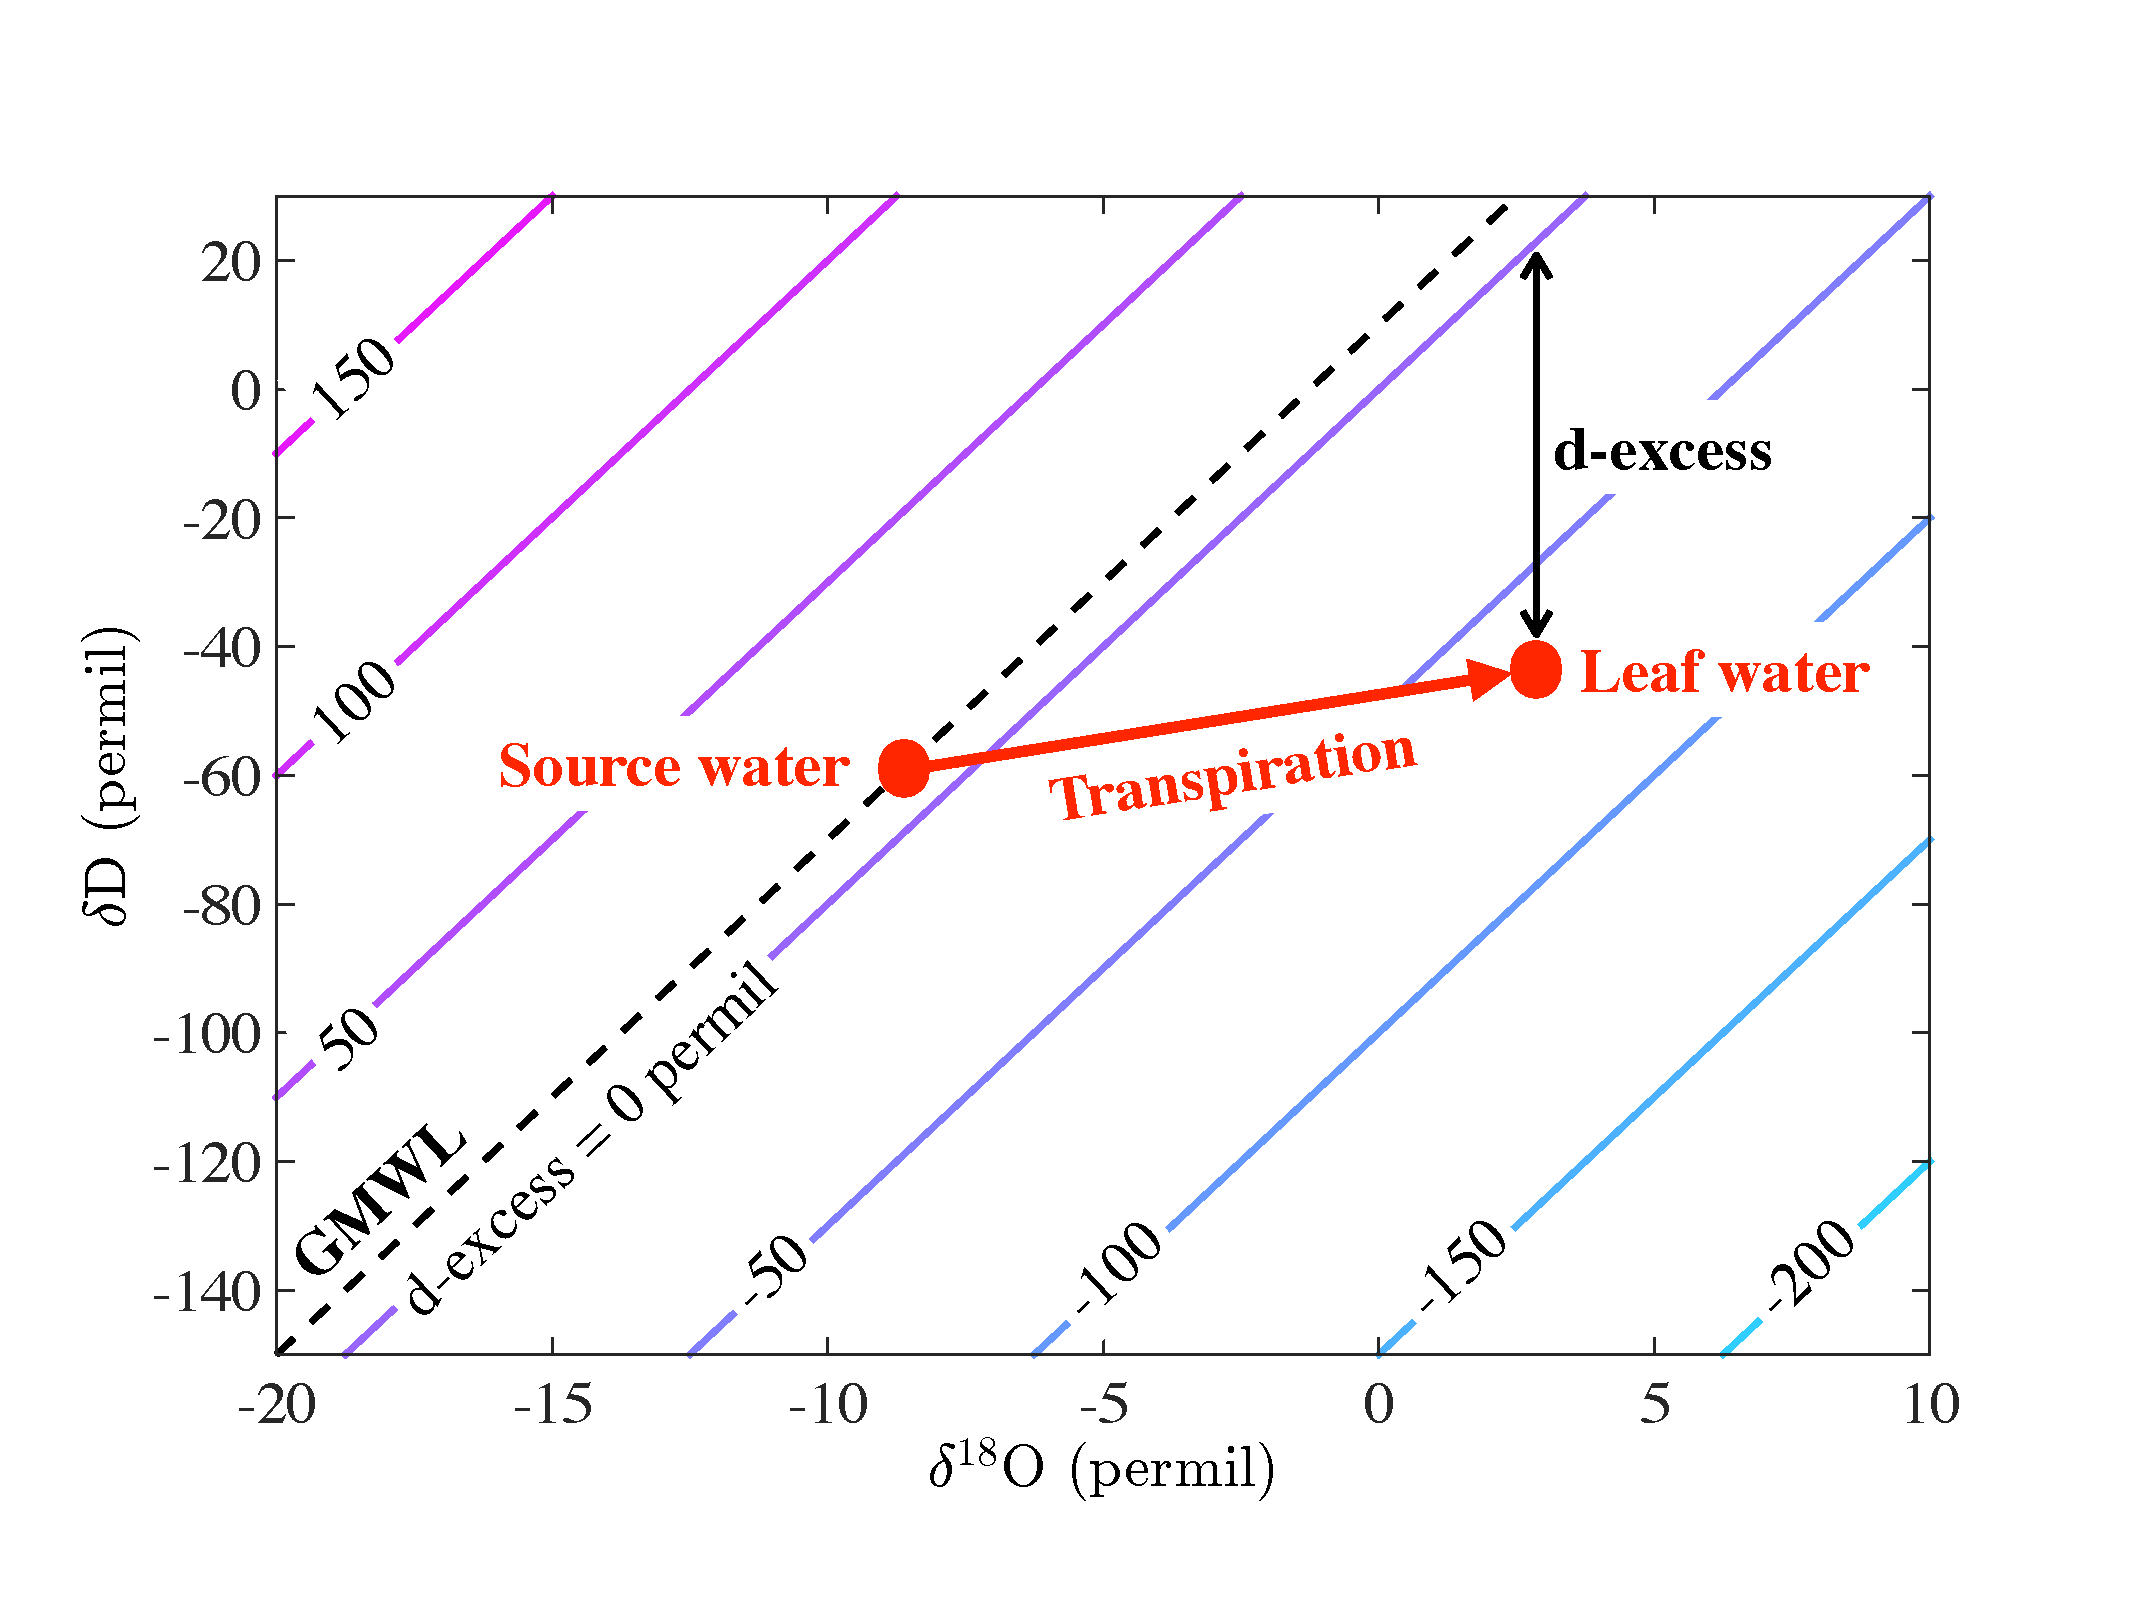
\includegraphics[width=\textwidth]{d18_dD_Concept_Final.pdf}
		\caption{Adapted from \cite{Voelker:2014bq}: Conceptual figure showing the evaporative conditions controlling the evolution of $\delta^{18}$O and $\delta$D in leaf water from source water located on the global meteoric water line (GMWL, dashed black line). The slope of the transpiration line depends on the relative humidity. The d-excess of a sample is the vertical distance from that sample to the d-excess reference line. The position of the source water along the GMWL depends on the temperature at which the water condensed and on the isotopic composition of the vapor.}\label{d18O_dD_Concept}
	\end{figure}
\end{center}

\begin{center}
	\begin{figure}
		\centering
		\includegraphics[width=\textwidth]{Final_d_excess_Plot.jpg}
		\caption{Maps of the spacial distribution of d-excess of five \textit{Colocasia esculenta} leaves collected throughout Experiment 1a. The maps were obtained by inverse distance interpolation of 12 to 25 sampling points analyzed on the Picarro Induction Module. All leaves are about 38~cm long. \textbf{Left:} initial leaf collected on day 0. \textbf{Top row:} leaves collected on day 14 (center) and 21 (far right) from the drought treatment. \textbf{Bottom row:} leaves collected on day 12 (center) and 21 (far right) from the sprayed treatment, where the leaves were sprayed with isotopically enriched water ($\delta^{18}$O = 8.85~\textperthousand, $\delta$D = 737.64~\textperthousand) every two days. The color scheme is the same for all rows and the values are expressed in permil.}\label{expe1a}
	\end{figure}
\end{center}

\begin{center}
	\begin{figure}
		\centering
		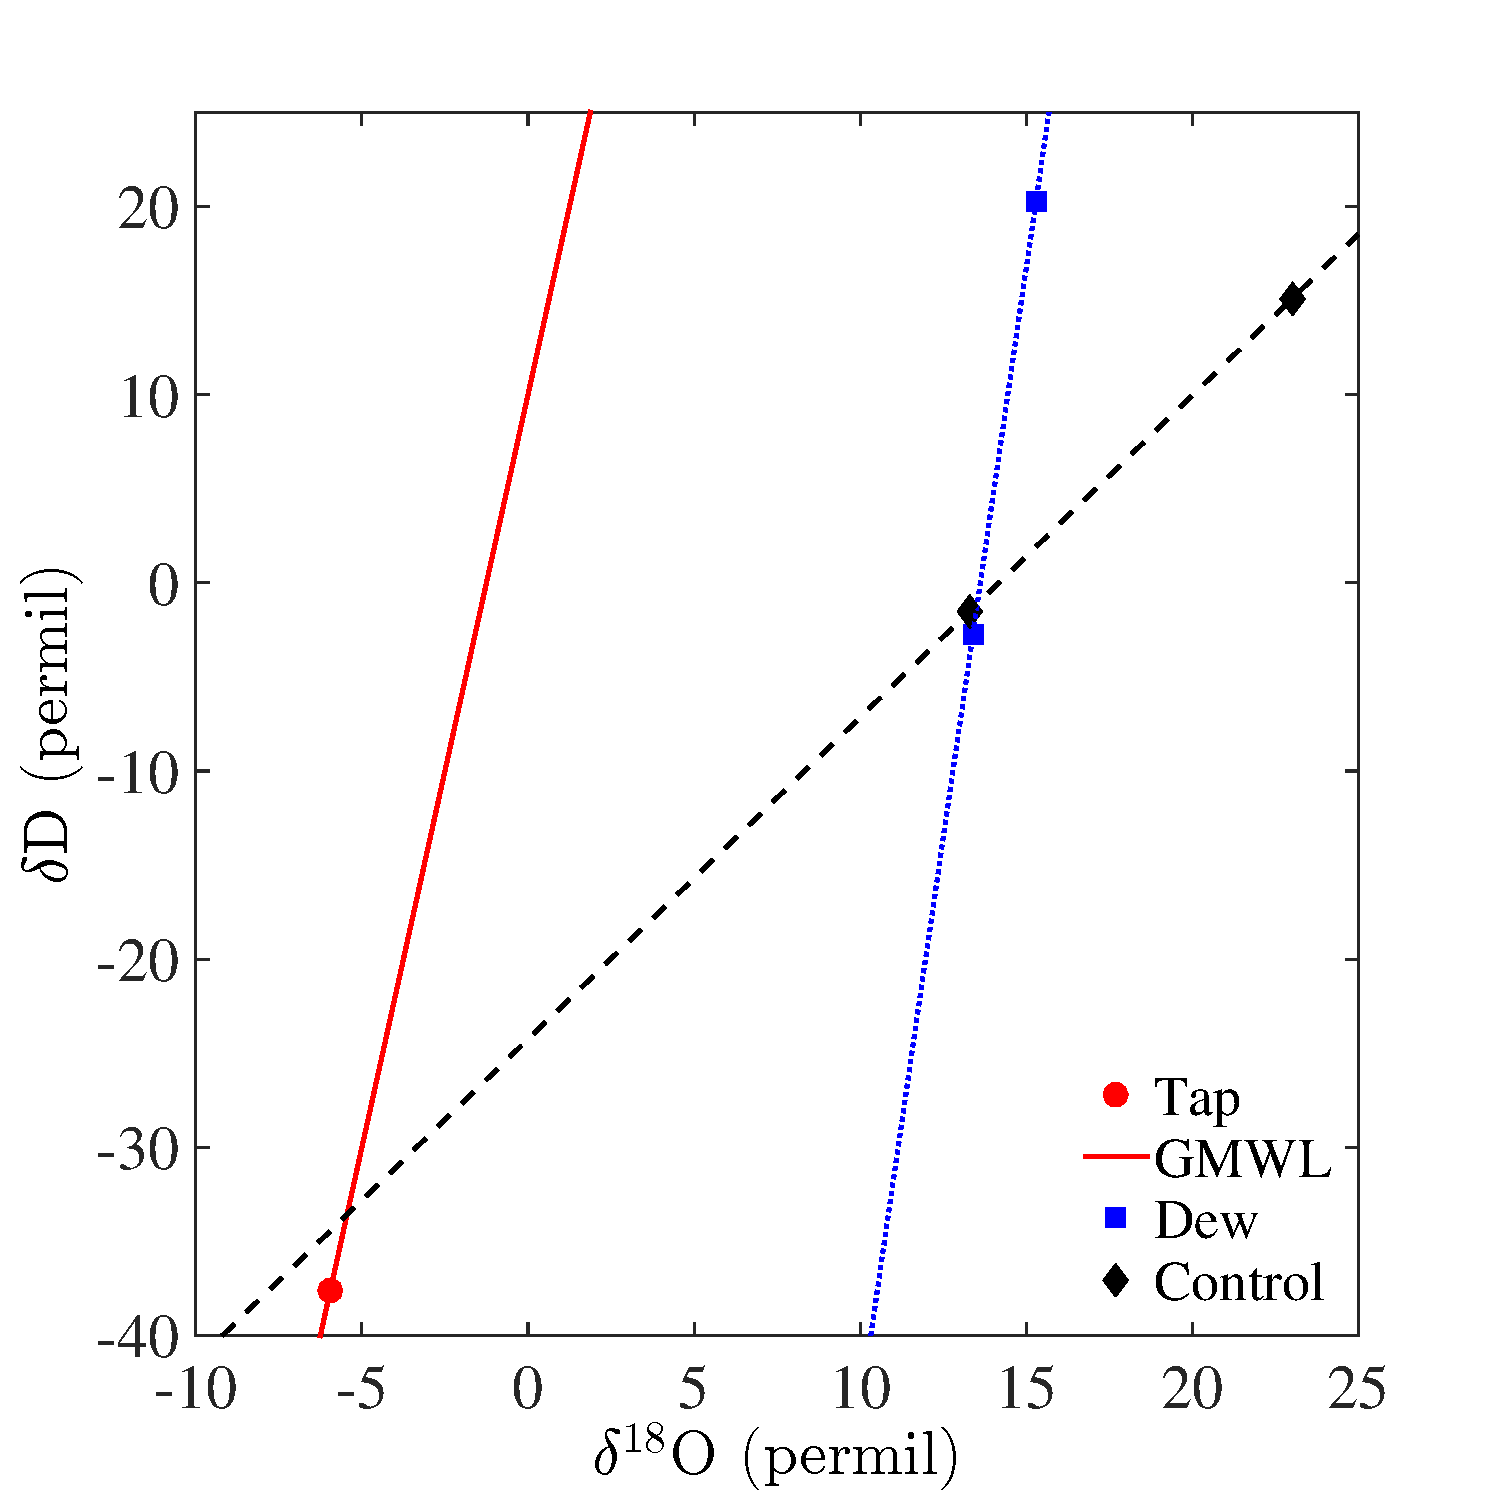
\includegraphics[width=0.8\textwidth]{d18_dD_Plot.pdf}
		\caption{Average $\delta^{18}$O and $\delta$D of four leaves analyzed in Experiment 1a. \textbf{Red circle:} Composition of the tap water used to water the plants during initial growth. \textbf{Red solid line:} Global meteoric water line (GMWL). \textbf{Blue squares:}  Isotopic composition of leaves collected on days 12 and 21 from the dew treatment, where the leaves were sprayed with isotopically enriched water ($\delta^{18}$O = 8.85~\textperthousand, $\delta$D = 737.64~\textperthousand) every two days. The blue dotted line shows the linear regression. \textbf{Black diamonds:} Isotopic composition of leaves collected on days 14 and 21 from the drought treatment. The black dashed line shows the linear regression. The drought treated leaves have a composition that corresponds to that of evaporated tap water, which was used to water the plants until maturation. The dew treated leaves are evolving on a line parallel to the GMWL, showing that transpiration almost completely stopped after the treatment began.}\label{d18O_dD}
	\end{figure}
\end{center}

\begin{center}
	\begin{figure}
		\centering
		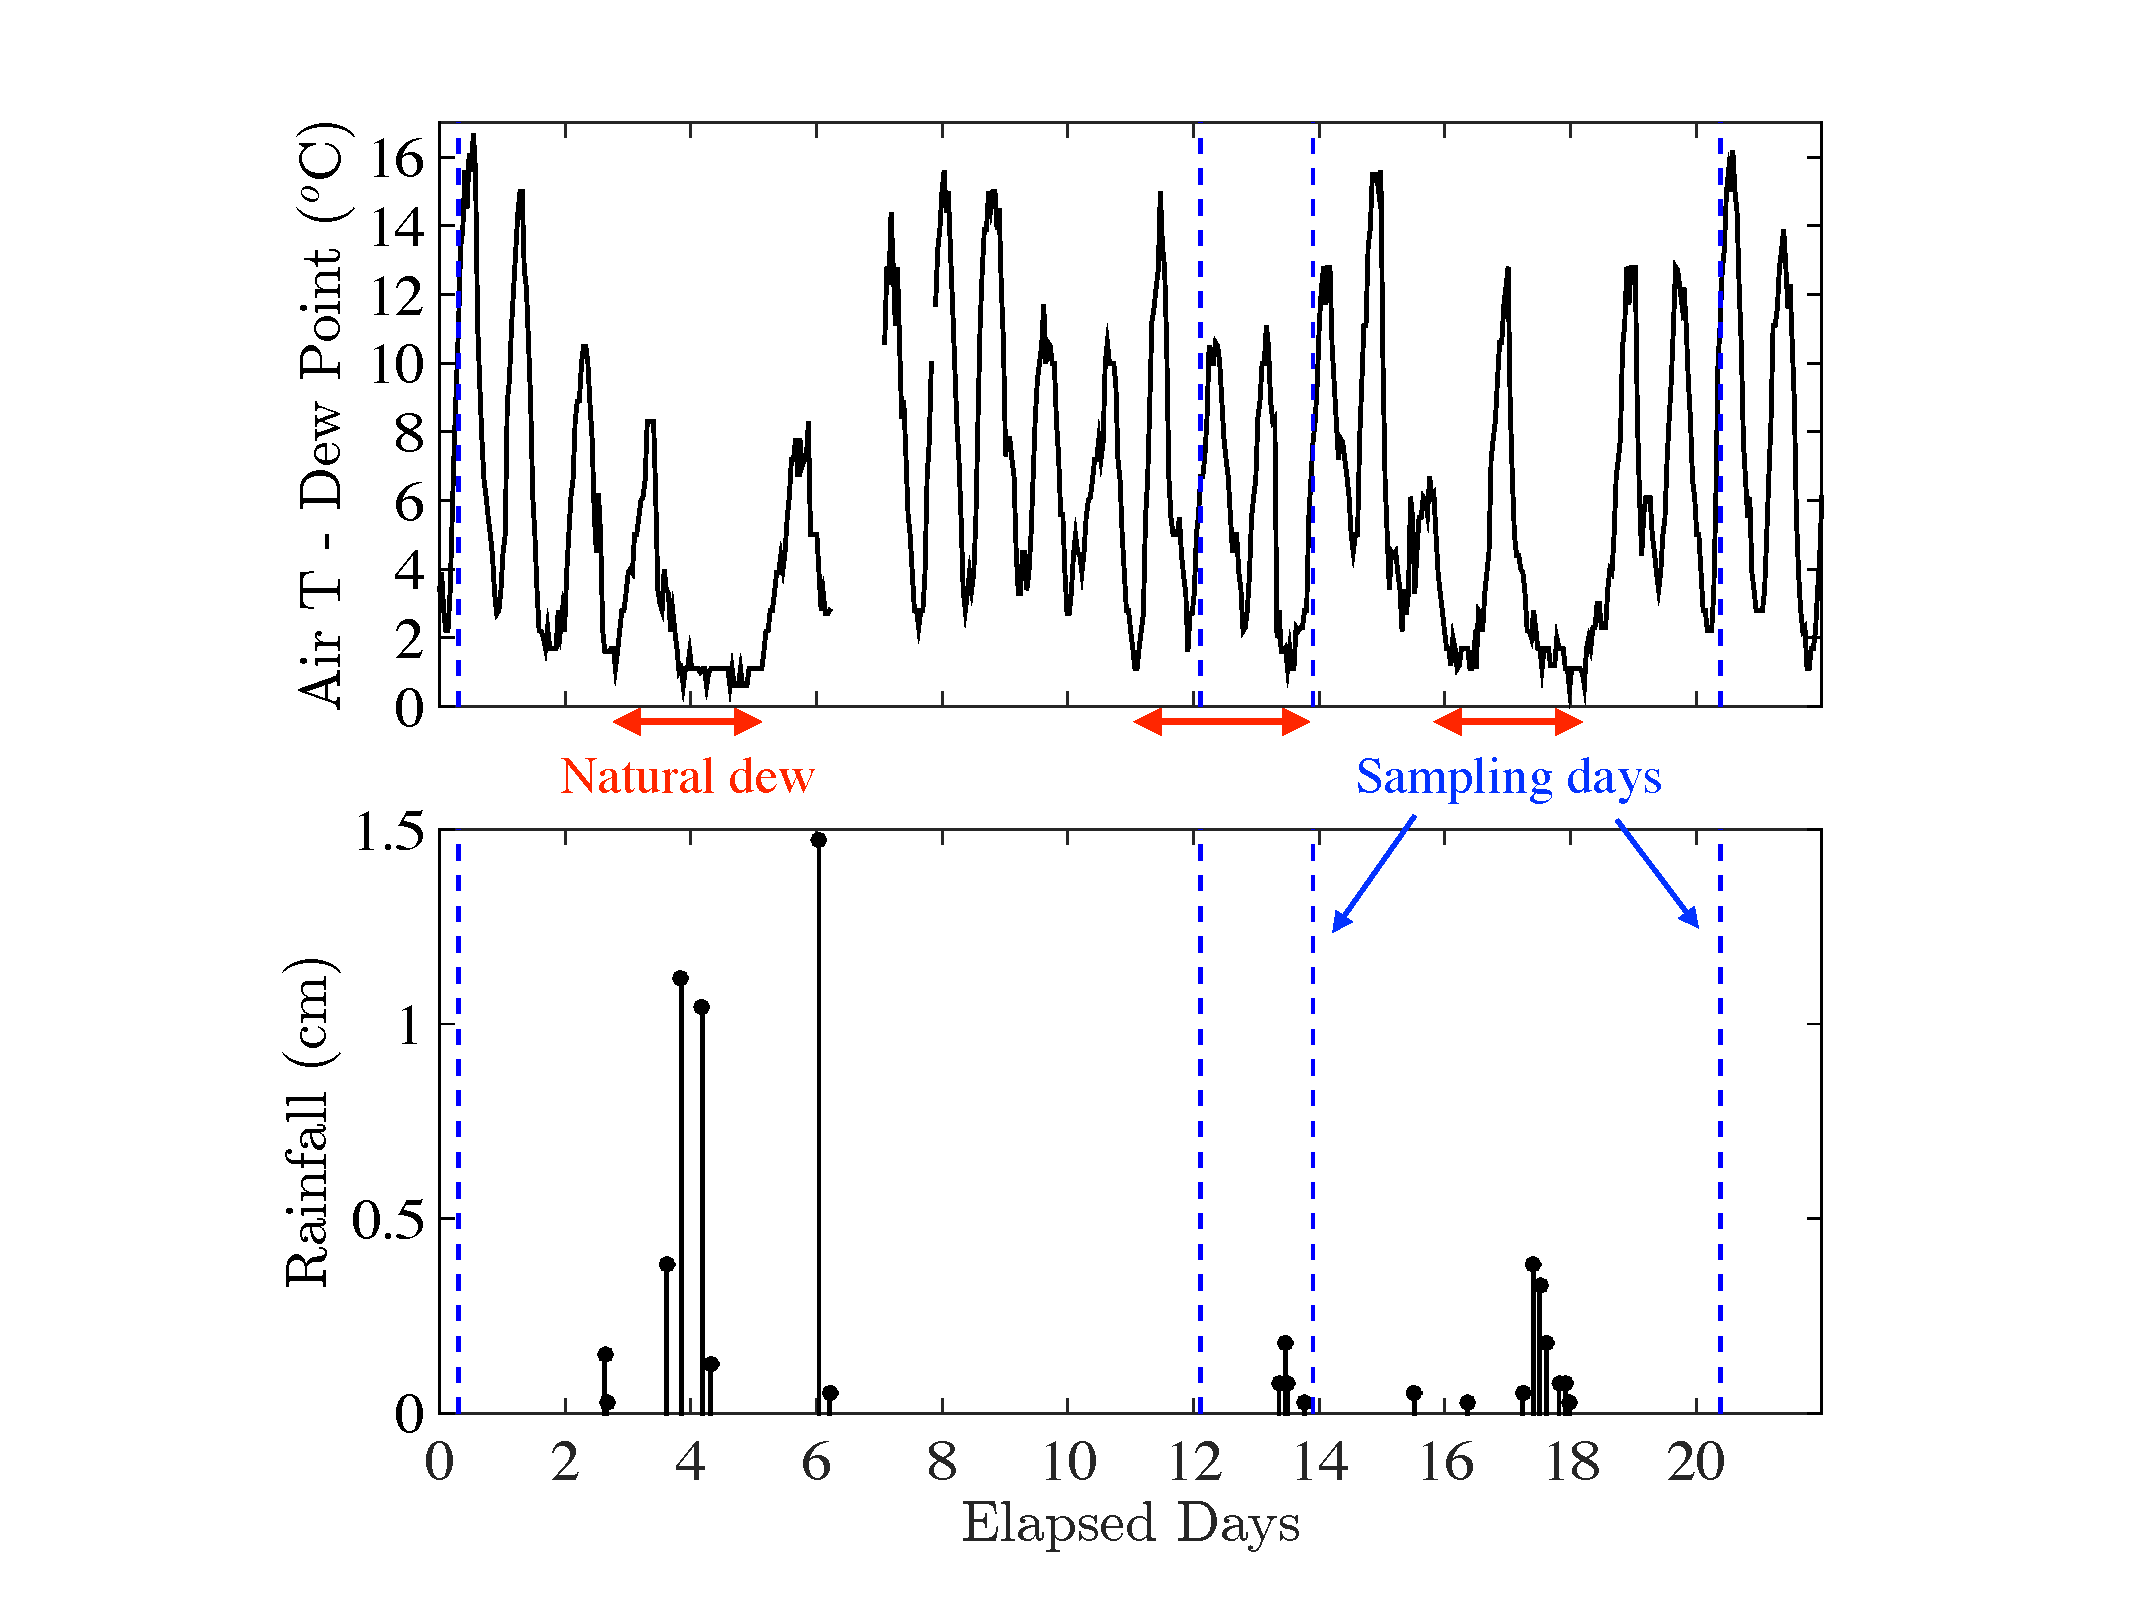
\includegraphics[width=\textwidth]{Experiment_DewPoint_T_Annotated.pdf}
		\caption{\textbf{Top panel:} Difference between the air and the dew point temperature over the course of the experiment ($^{\text{o}}$C). \textbf{Bottom panel:} Rainfall (cm) over the course of the experiment. The blue dashed vertical lines mark the days of collection: the initial leaf was collected on day 0, leaves from the dew treatment were collected on days 12 and 21 and leaves from the drought treatment were collected on days 14 and 21. Red horizontal arrows indicate days when the leaves most likely experienced natural dew deposition because of the local air temperature and relative humidity under the sheltered area. The collection of the first dew treated leaf happened right after a series a small rain events and four nights in a row of temperatures close to the dew point temperature.}\label{dewpoint}
	\end{figure}
\end{center}
\begin{center}
	\begin{figure}
		\centering
		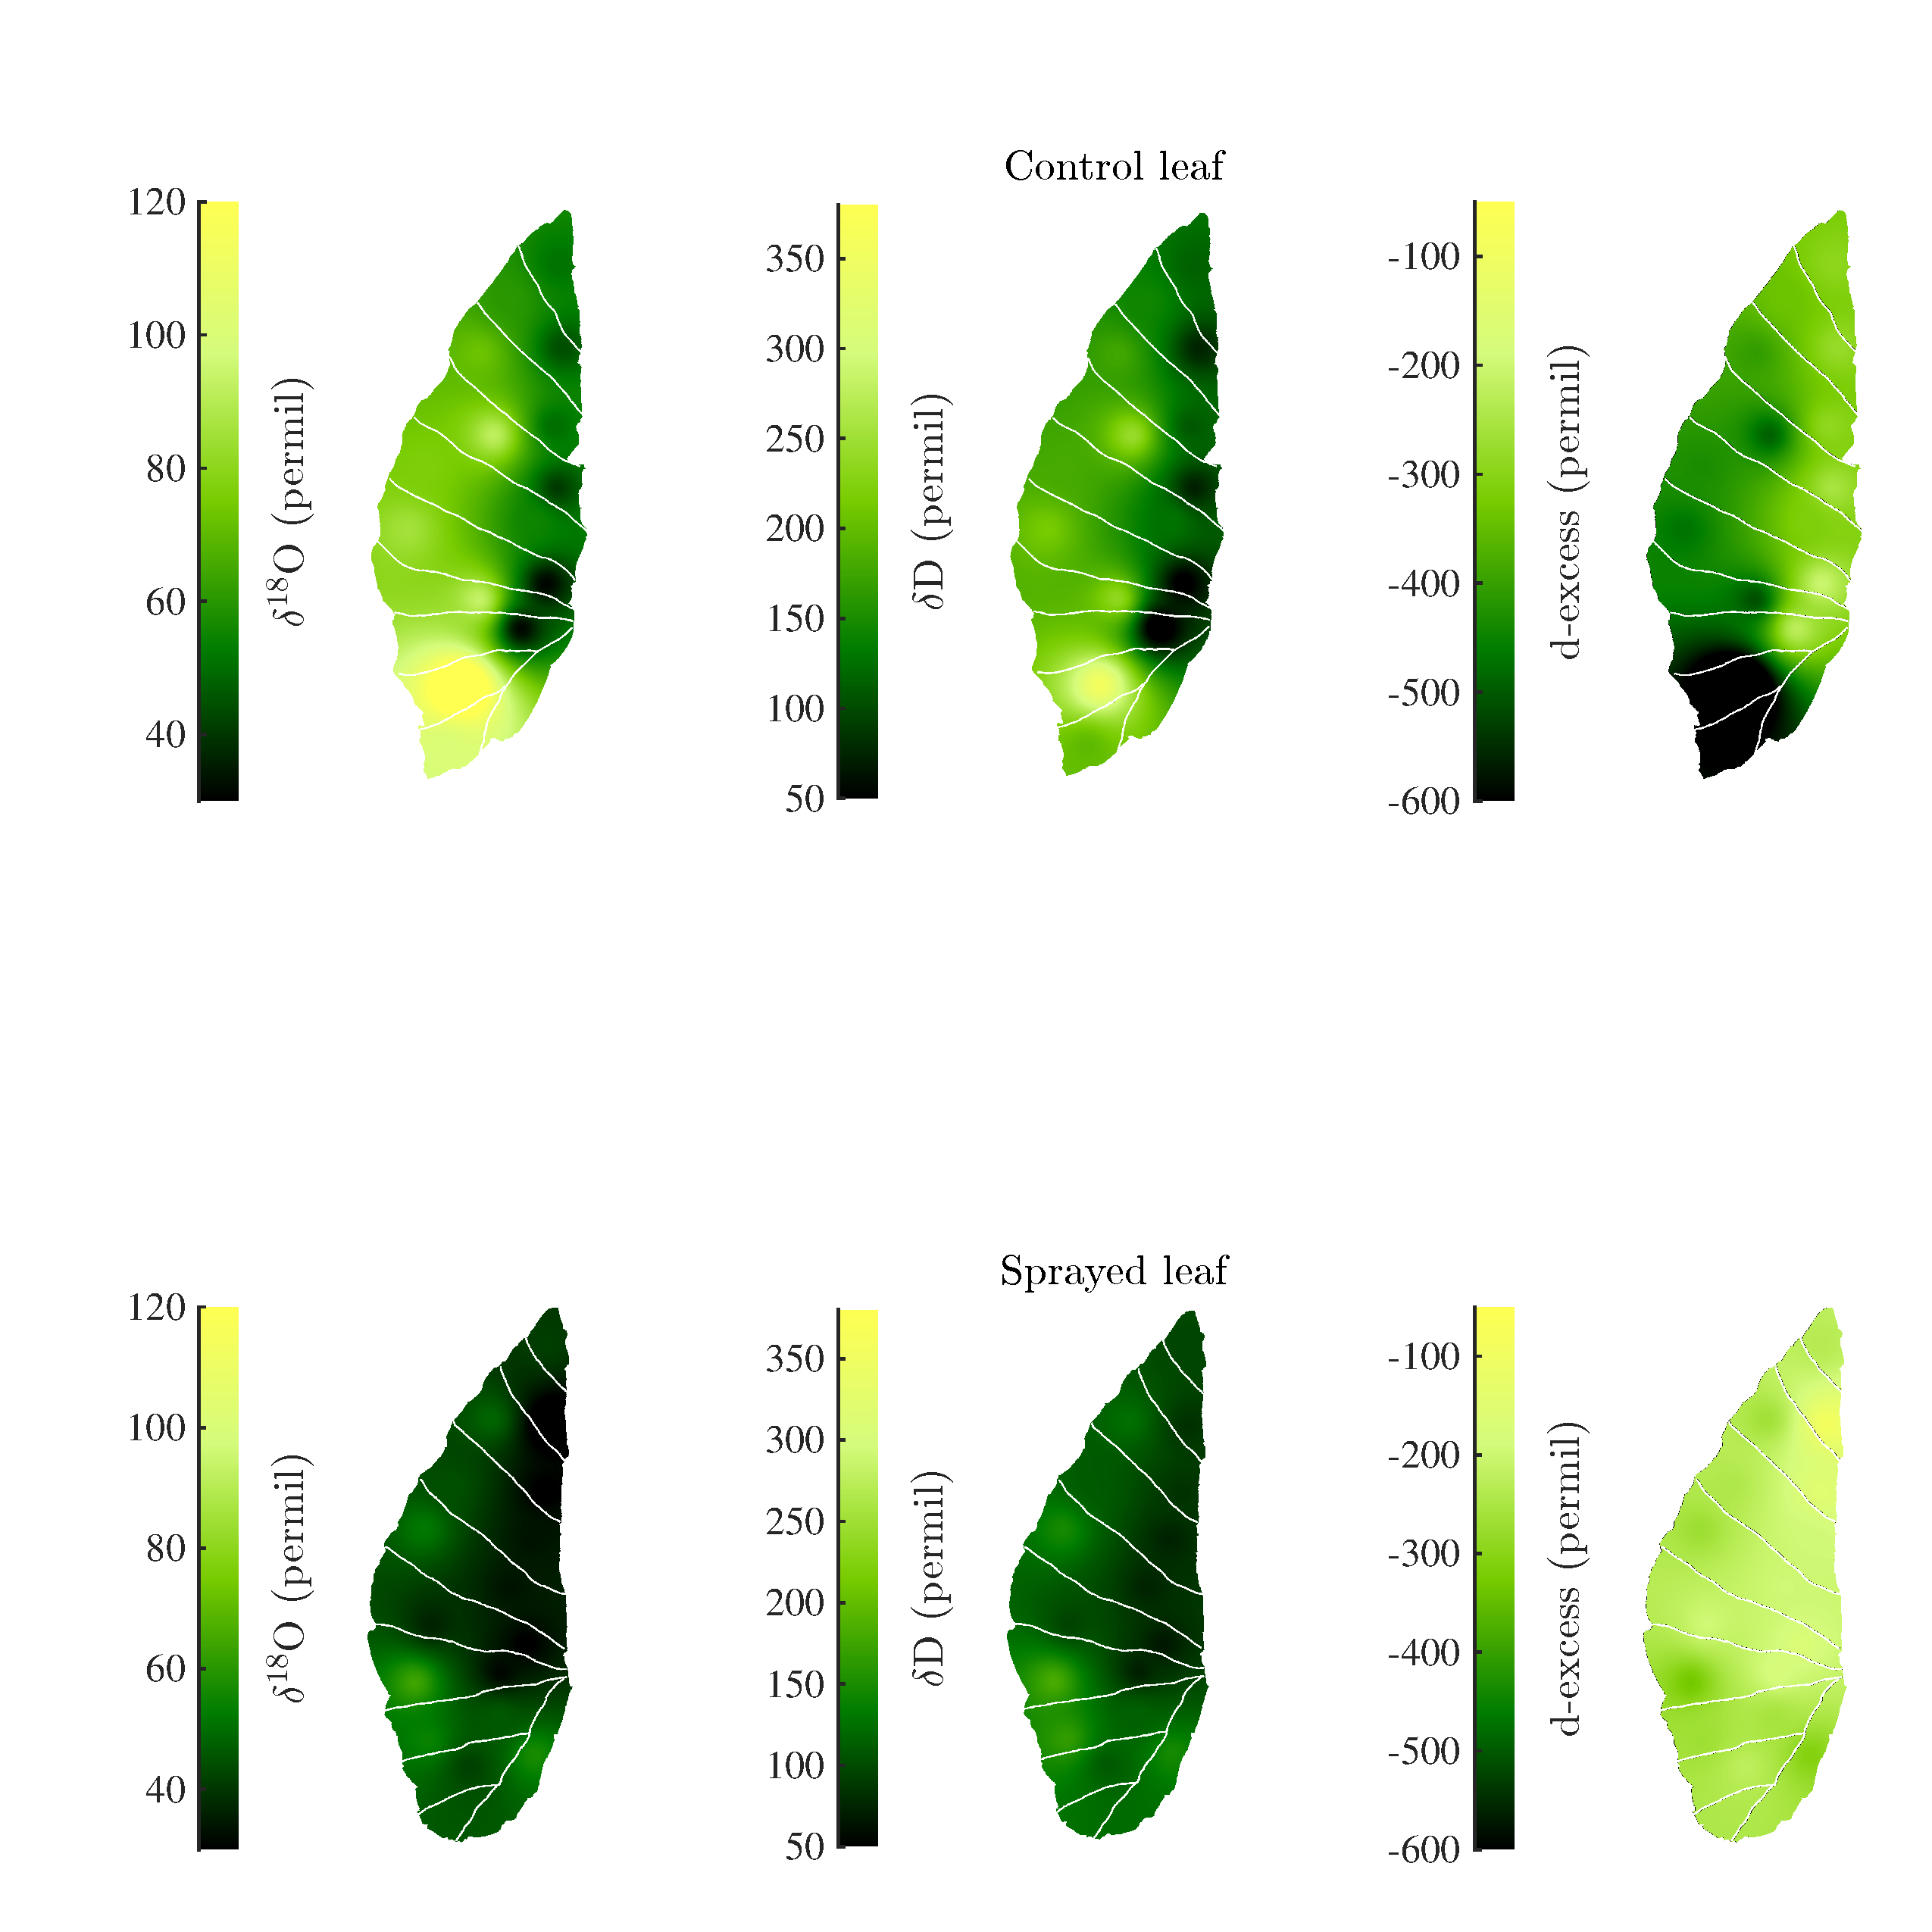
\includegraphics[width=\textwidth]{Dec1stExpe.pdf}
		\caption{Maps of two leaves left to dry under a 500W blue light for four hours. \textbf{Top row:} $\delta^{18}$O, $\delta$D and d-excess of the non-sprayed leaf. \textbf{Bottom row:} $\delta^{18}$O, $\delta$D and d-excess of the leaf sprayed with isotopically enriched water ($\delta^{18}$O = 8.85~\textperthousand, $\delta$D = 737.64~\textperthousand) every half-hour. The non-sprayed leaf shows higher enrichment and lower d-excess values that are associated with increased transpiration compared to the sprayed leaf.}\label{expe1b}
	\end{figure}
\end{center}
\begin{center}
	\begin{figure}
		\centering
		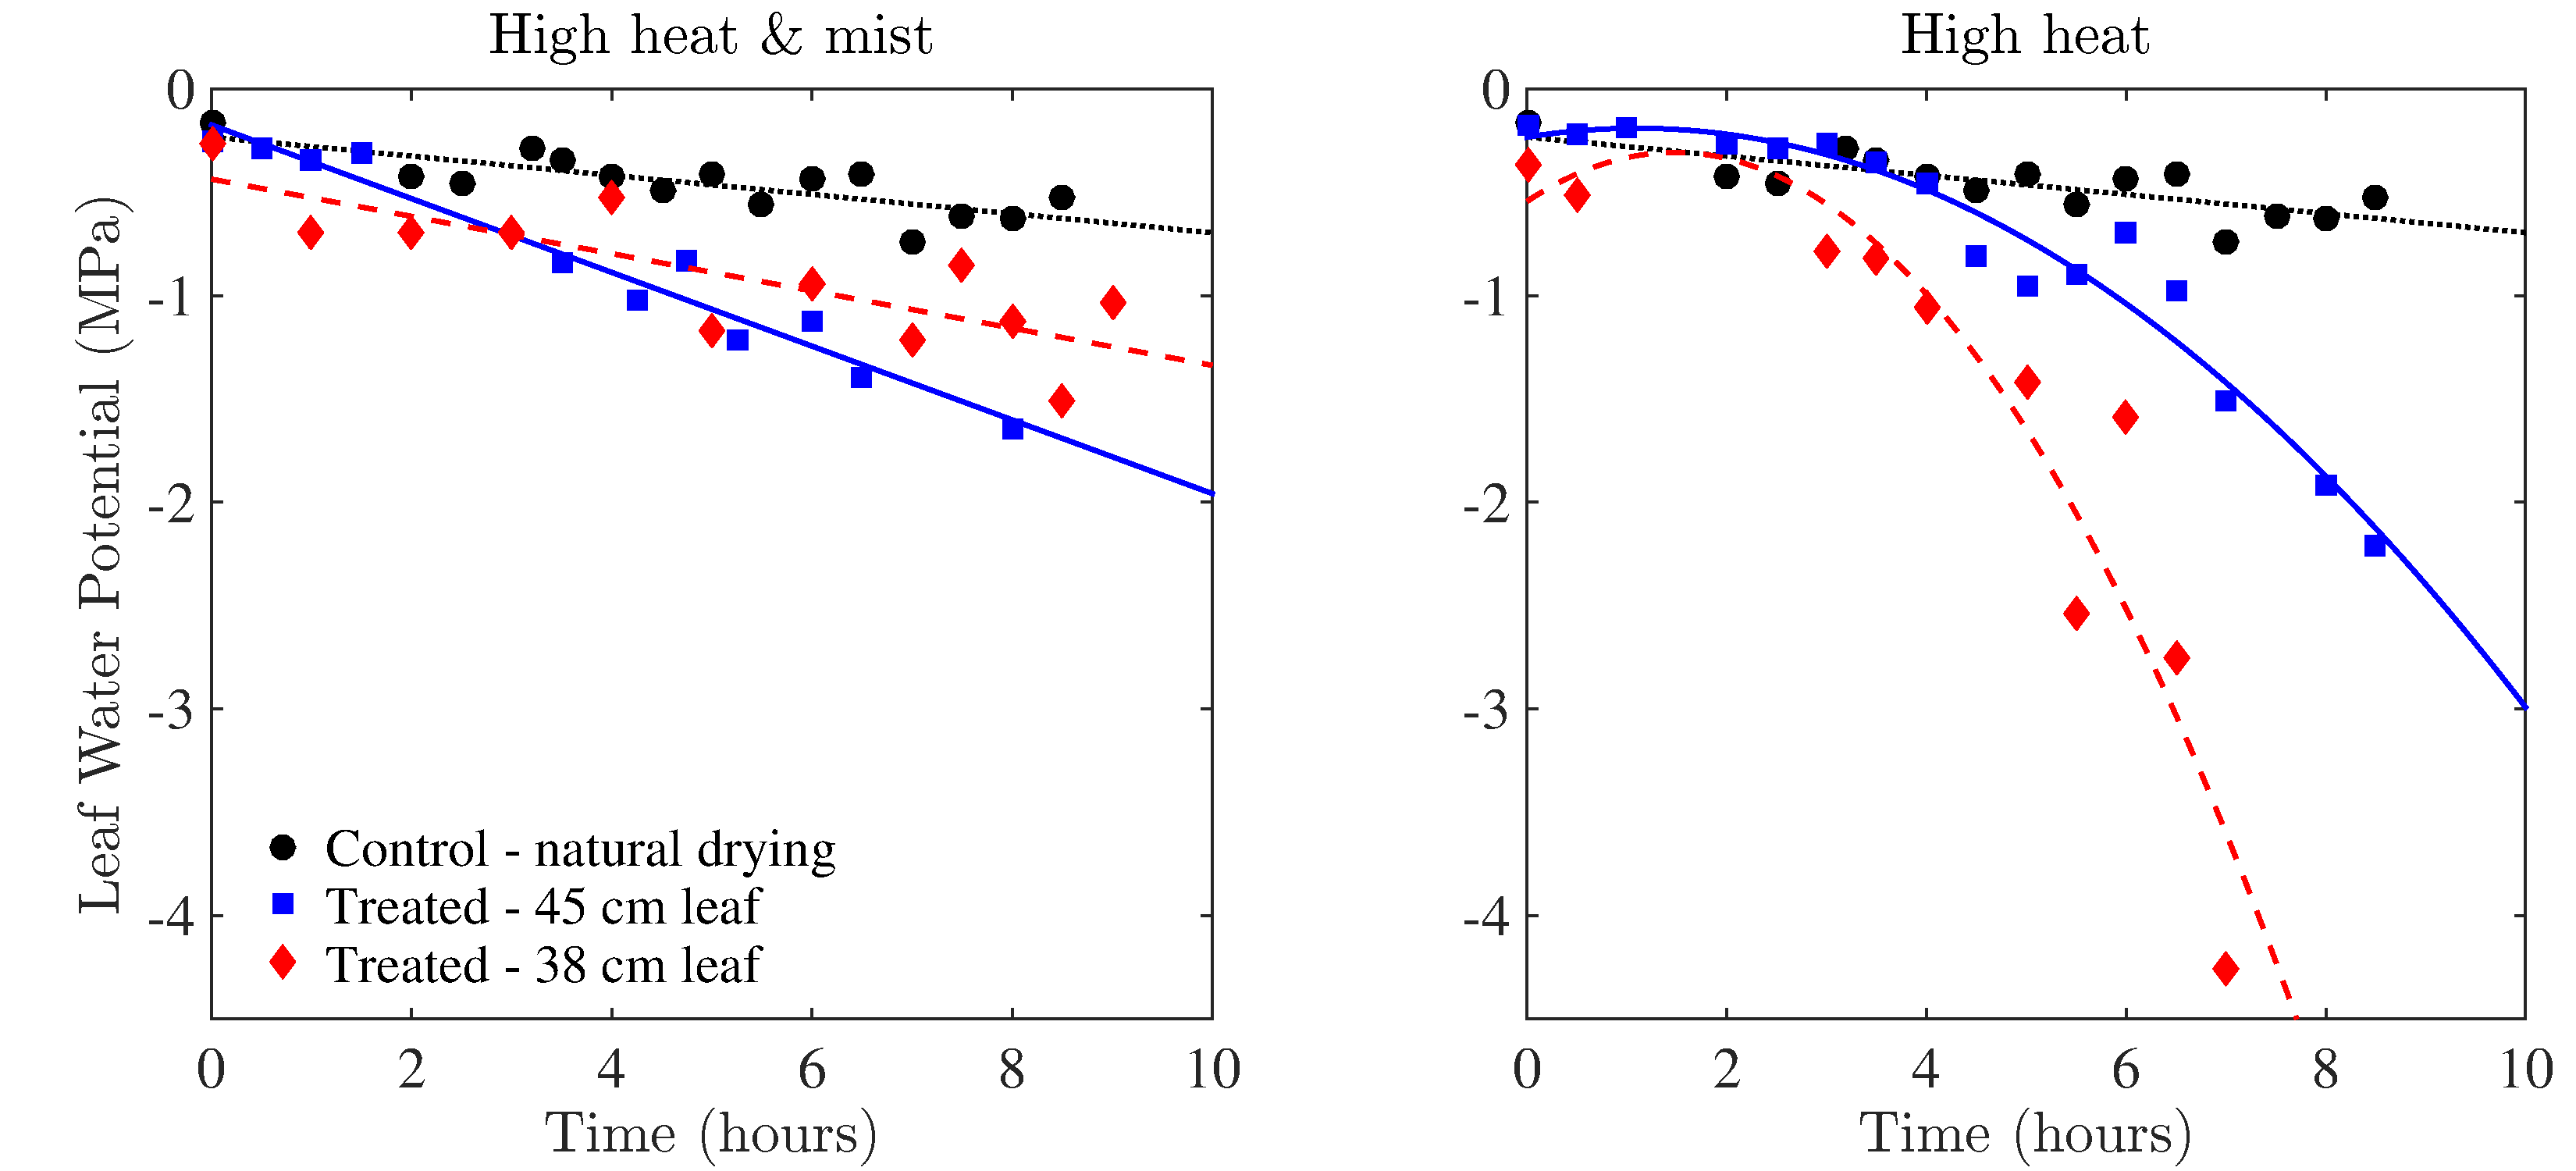
\includegraphics[width=\textwidth]{Dryout_Expe.pdf}
		\caption{Five examples of the temporal evolution of leaf water potential of \textit{Colocasia esculenta} leaves. The red diamonds are 38~cm long leaves. All other leaves are 45~cm long (black and blue). On the left, natural drying (black dotted line) and both sizes leaf in the high heat \& mist (red dashed and blue solid lines) case are best fitted by a linear relation. On the right, the high heat drying case is best fitted by a parabola for both 38 (red dashed line) and 45 cm (blue solid line) leaves.}\label{expe2}
	\end{figure}
\end{center}
\begin{center}
	\begin{figure}
		\centering
		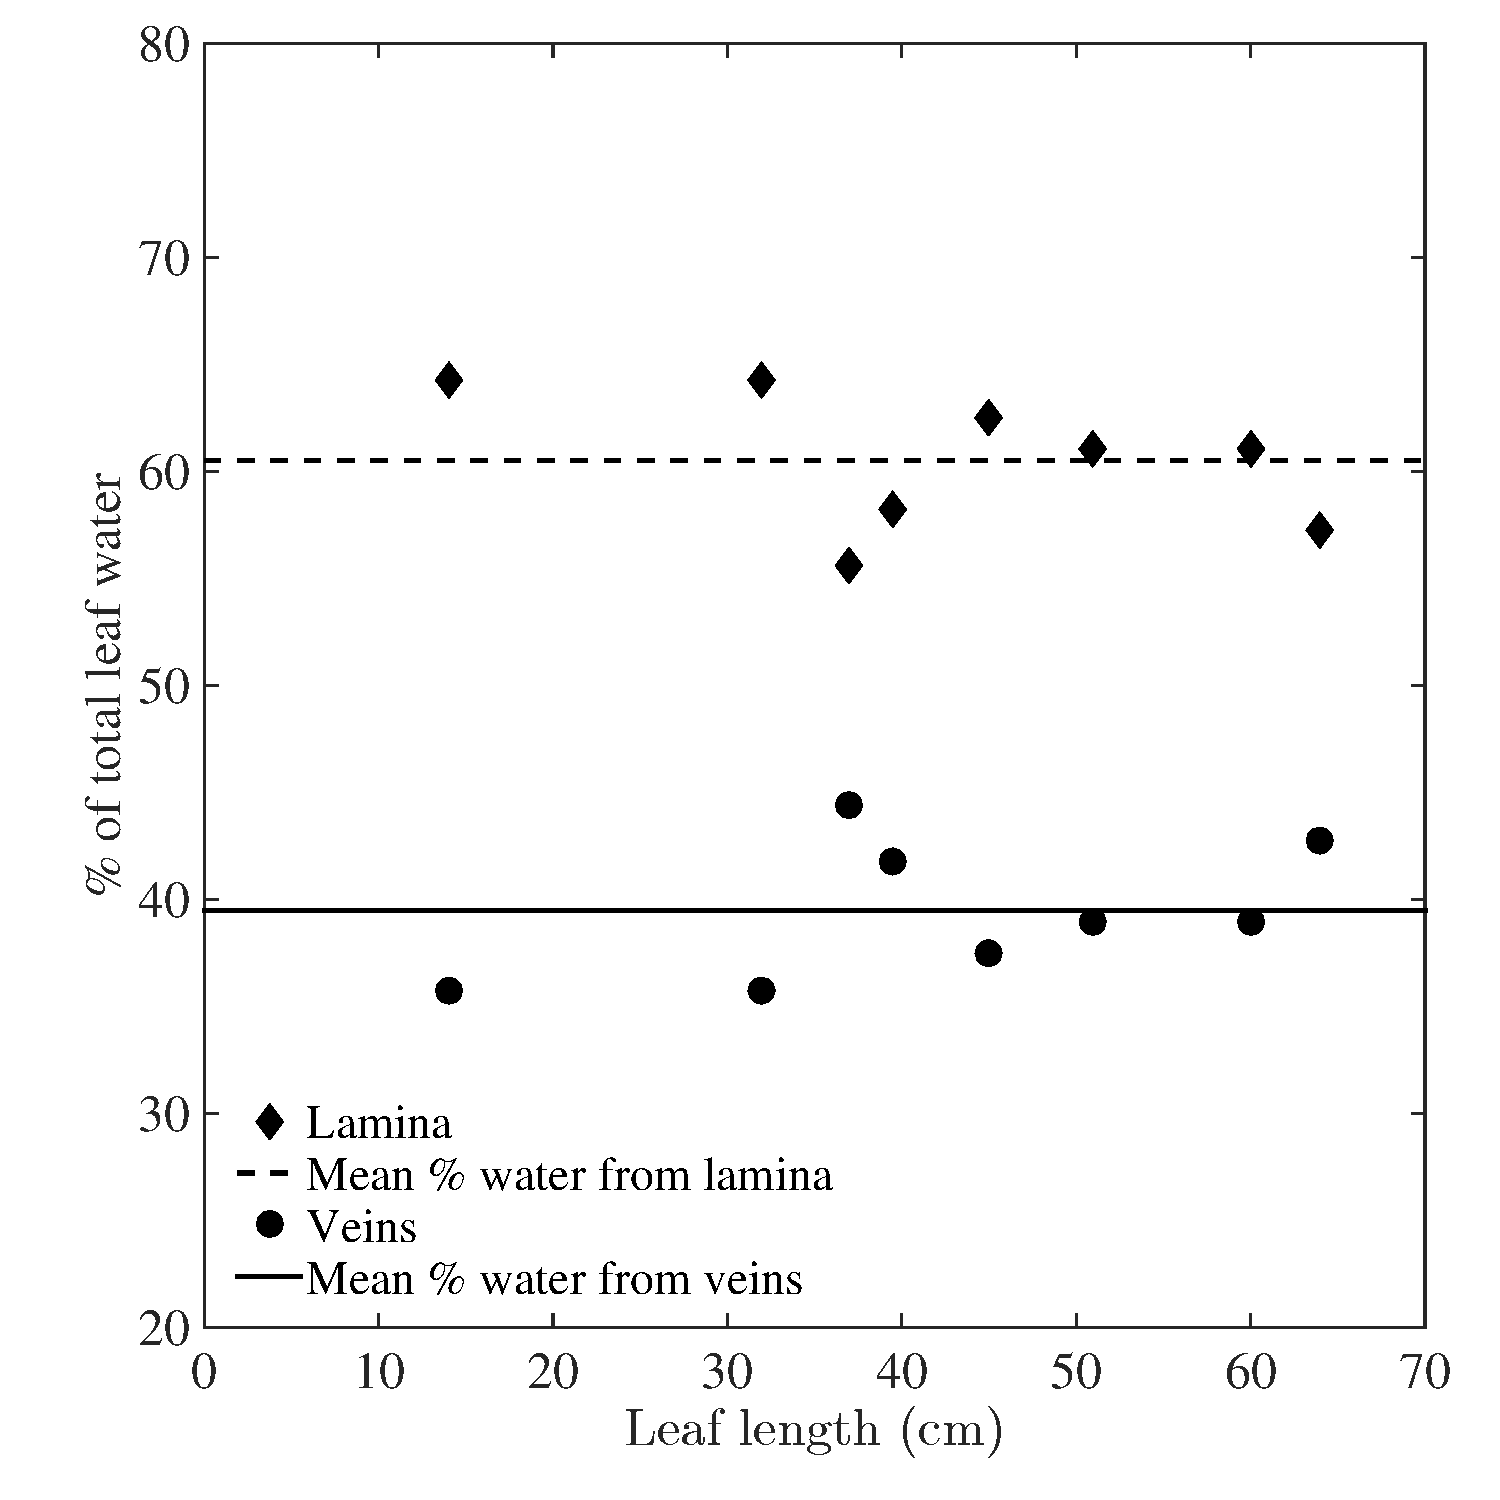
\includegraphics[width=0.5\textwidth]{Vein_Tissues.pdf}
		\caption{Percent water from veins and lamina for eight leaves of \textit{Colocasia esculenta} with lengths ranging from 14 to 64 cm. \textbf{Red squares:} \% water from the lamina (dashed red line represents the mean value). \textbf{Black circles:} \% water from the veins (solid black line represents the mean value). On average, veins accounted for 39\% and the lamina for 41\% of the total water content of the leaves. The repartition of leaf water between the veins and the lamina shows no significant correlation with leaf size.}\label{waterPercent}
	\end{figure}
\end{center}
\newpage
%----------------------------------------------------------------------------------------
%10. Supplemental data files.
%----------------------------------------------------------------------------------------


\end{document}
